\documentclass[
final,
babelLanguage=british,
desktopVersion,
% showtrims,
% overleaf,
]{anecdote}

\graphicspath{{./assets/photos/300dpi/}}

% Page size: 210mm x 148mm (A5)
% Body text: 12.5 / 18 pt

\usepackage{local}

%%%%%%%%%%%%%%%% Details of the Book %%%%%%%%%%%%%%%%

\title{Thai Dhammayut Bhikkhupātimokkha}
\subtitle{Monk Training Centre}
\author{SBS Saṅgha}
\publisher{Sāsanārakkha Buddhist Sanctuary}
\date{2021-10-30}% chktex 8
\editionInfo{\textit{First edition}, 2022}
\ISBN{000-0-00000-000-0}

%%%%%%%%%%%%%%%% Metadata %%%%%%%%%%%%%%%%

\hypersetup{
  pdftitle={\thetitle},
  pdfauthor={\theauthor},
  pdfcopyright={Copyright (C) 2022, \thePublisher},
  pdfsubject={},% subject
  pdfkeywords={},% keywords
  pdflicenseurl={https://creativecommons.org/licenses/by-nc-nd/4.0/},
  pdfcontacturl={},
  pdflang={en},
}

%%%%%%%%%%%%%%%% Load Further Packages  %%%%%%%%%%%%%%%%

% Adds the time to version creation.
\usepackage[yyyymmdd,hhmmss]{datetime}
% \usepackage{titlesec}

% Using memoir's endnotes, called pagenotes
\makepagenote
\continuousnotenums

%%%%%%%%%%%%%%%% Hyphenation Exceptions and Corrections   %%%%%%%%%%%%%%%%

\hyphenation{London re-lin-quishes de-ter-mines}

\openany%

\begin{document}

\frontmatter

\ifdesktopversion
\desktopCover{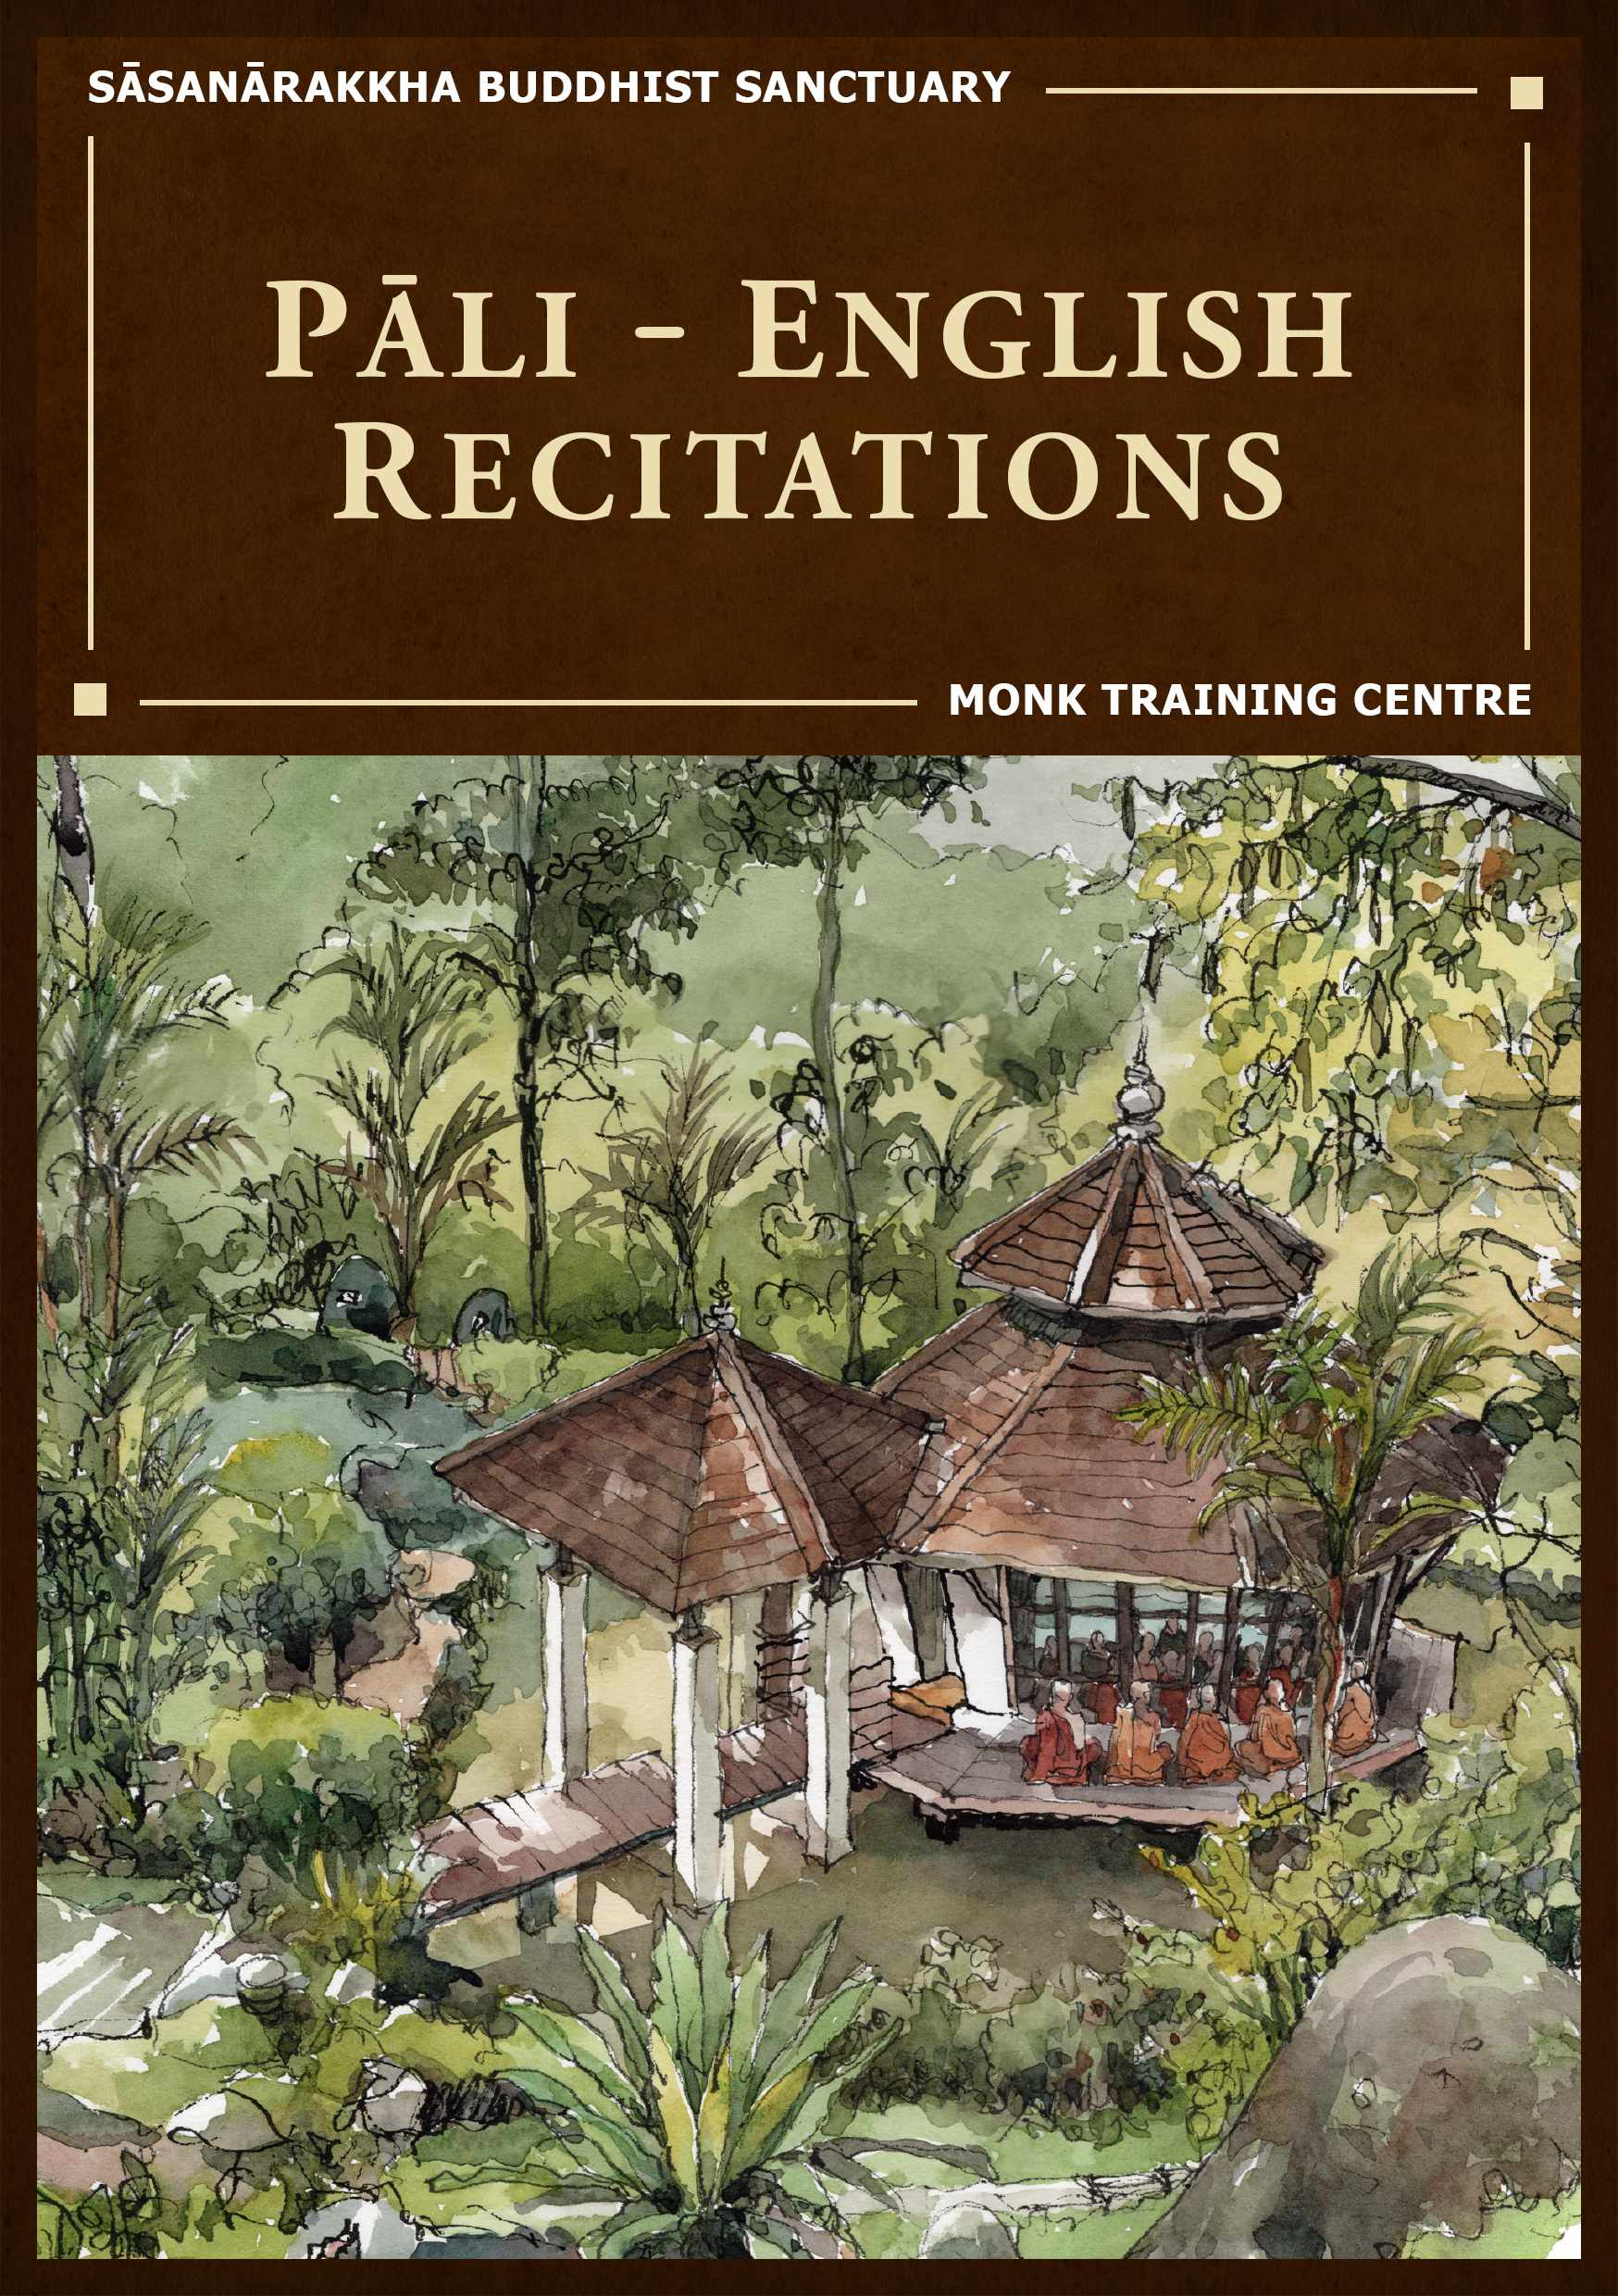
\includegraphics[height=\paperheight]{./front-cover-compressed.jpg}}
\fi

\pagestyle{empty}
\cleartorecto
\thispagestyle{empty}
\vspace*{3em}

{\centering

  \settowidth{\titleLength}{%
    {\Large\chapterTitleFont\textsc{\MakeUppercase{{\thetitle}}}}%
  }

  % 'SBS' on title page
  {\Huge\fontsize{64}{16}\sbsFont SBS}\\[1.0\baselineskip]%

  % 'Monk Training Centre'
  {\Huge\chapterTitleFont\textsc{{\thesubtitle\linebreak}}}\\[0.2\baselineskip]
  \setlength{\xheight}{\heightof{X}}

  % Ornament
  \raisebox{0.5\xheight}{\pgfornament[color=sbs-brown,width=7cm,scale=1,ydelta=0pt,symmetry=c]{84}}\\[1.4\baselineskip]

  % 'Pali-English Recitations'
  {\Large\scshape \thetitle}\\[2.5\baselineskip]

  % Dhamma quote
  {\quote ``The Blessed One who knows and sees, accomplished and fully enlightened, has prescribed the course of training for bhikkhus and he has laid down the Pātimokkha. On the Uposatha day as many of us as live in dependence upon a single village district meet together in unison, and when we meet we ask one who knows the Pātimokkha to recite it. If a bhikkhu remembers an offence or a transgression while the Pātimokkha is being recited, we make him act in accordance with the Dhamma, in accordance with the instructions. It is not the worthy ones that make us act; it is the Dhamma that makes us act.''\\ \smallskip (MN 108)}\\[1.4\baselineskip]
}

\cleartoverso
\thispagestyle{empty}

\vspace*{-\baselineskip}

{%

\fontsize{10}{16}\selectfont
\centering
\setlength{\parindent}{0pt}%
% \setlength{\parskip}{0.8\baselineskip}%

\vspace{0.5cm}

Published by TBD\\
% TODO need 2 ISBN numbers assigned (1 for print/pdf, 1 for epub); do more research before printing
% https://www.pnm.gov.my/
ISBN \theISBN\\
Copyright \copyright\ Sāsanārakkha Buddhist Sanctuary 2022

\vspace{0.5cm}

This book is for free distribution only;\\
it may not be sold.

\vspace{0.5cm}

Download this book as a PDF, EPUB, or MOBI\\
at the following address:\\
\href{https://sasanarakkha.org/}{https://sasanarakkha.org}

\vspace{0.5cm}

Project Manager: Ā. Ariyadhammika\\
Editor: Ā. Pāladhammika\\
Typesetting: Aj. Gambhiro, Ā. Pāladhammika\\
Translators: Ā. Ñāṇatusita\\
Endnotes: Ā. Ariyadhammika, Ā. Ṭhānissaro

\vspace{0.5cm}

This work is licensed under a Creative Commons\\
Attribution-NonCommercial-NoDerivatives 4.0 International~License.

Produced with the \LaTeX\ typesetting system,\\
set in Libertinus Serif.

\vspace{0.5cm}

\ifdesktopversion
This version was created on:\\
\today \space at \currenttime
\fi

\vspace{0.5cm}


\theEditionInfo

}

% \cleartorecto
\thispagestyle{empty}

{\setlength{\parskip}{10pt}

{\centering\fontsize{20}{25}\selectfont
\textsc{We Wish To Gratefully Acknowledge}
\par}

The Saṅghas of Wat Pah Nanachat (WPN), Amaravati, and Abhayagiri for allowing the use of material from their respective chanting books, the late Ven. Dr. Saddhātissa and Mr. Maurice Walshe for their English translations, as well as Ven. Bhikkhu Bodhi for granting permission to use and slightly adapt his translations. Further contributions are found on the previous page.

\vspace*{1.5\baselineskip}

Additional information on translations, as well as deviations\pagenote{%
  Due to the balanced and inspiring selction of chants, as well as for the sake of
  compatibility, the WPN chanting book has served as the basis for the SBS
  chanting book. Over time, suggestions for the inclusion of additional chants, as
  well as occasional improvements of existing translations were incorporated. Such
  changes were meticulously marked down in the endnotes, so that someone familiar
  with the SBS chanting book can straight away find the relevant differences,
  which can be useful when visiting a branch monastery of the Ajahn Chah lineage,
  in order to know in which places to revert to the original version.}
from WPN Chanting Book (2014), have been annotated by Ven. Ariyadhammika in the endnotes.

\bigskip

{\centering
To Āyasmā Aggacitta, the founding father of\\
Sāsanārakkha Buddhist Sanctuary.

\bigskip

\includegraphics[height=65mm]{SBS_logo_Tuck_Loon_BAedit_2020_small.jpg}

}

}


\cleartorecto
\pagestyle{toponerow-frontmatter}
\chapterstyle{adrasteia-toc}

\pdfbookmark[section]{\contentsname}{toc}
\tableofcontents*

% \section{Abbreviations}

% \thispagestyle{empty}

% {\subsectionFmt{Abbreviations used in the text}}
% \bigskip

% {\raggedright
% \fontsize{10}{14}\selectfont

\begin{center}
  \begin{tabular}{@{}lll@{}}
    % [...  \hspace{-0.5mm}\anglebracketright\ & = & Only recited by the leader \\
    \breathmark\ & = & Take a breath \\
  \end{tabular}

  % Wisdom Publication sources: Nikāya and sutta # (eg. DN 1)
  % P.T.S. sources: Nikāya, volume #, page # (eg. D i 1)

  \begin{tabular}{@{}ll@{}}
    Vin   & Vinaya Piṭaka           \\
    DN    & Dīgha Nikāya            \\
    MN    & Majjhima Nikāya         \\
    SN    & Saṁyutta Nikāya         \\
    AN    & Aṅguttara Nikāya        \\
    Khp   & Khuddakapāṭha           \\
    Dhp   & Dhammapada              \\
    Ud    & Udāna                   \\
    Snp   & Sutta Nipāta            \\
    Thag  & Theragāthā              \\
    Ja    & Jātaka                  \\
    Ps    & Paṭisambhidāmagga       \\
    Vibh  & Abhidhamma Vibhaṅga     \\
    A     & Aṭṭhakathā              \\
    Dhs   & Dhammasaṅganī           \\
    A     & Aṭṭhakathā              \\
    A     & Aṭṭhakathā              \\
    MJG   & Mahā-jaya-maṅgala-gāthā \\
    Thai  & Composed...             \\
    Sri L & Composed...             \\
    Trad  & Tradtional...           \\
  \end{tabular}
\end{center}

% \bigskip

% Wisdom Publication sources: Nikāya and sutta # (eg. DN 1)
% P.T.S. sources: Nikāya, volume #, page # (eg. D i 1)

% References to shorter texts consisting of verses such as the Dhammapada, Udāna,
% Itivuttaka, Theragāthā, Therīgāthā or Sutta Nipāta are to the verse number or
% chapter and verse number. The other longer texts are referred to by volume and
% page number of the PTS edition.

% }


\chapterstyle{adrasteia-frontmatter}

\mainmatter
\pagestyle{toponerow}

\cleartorecto
% \part{Pāli}

{\raggedright
  \chapterOpeningPage{appendix-compressed.jpg}

% TODO change to pali.jpg

\chapter{Pāli}

\clearpage

\section{Pubbakicca}
\label{pubbakicca}

\linkdest{endnote13-body}
\begin{intro}
  Okāsaṁ me bhante thero detu pāṭimokkhaṁ uddesituṁ.\makeatletter\hyperlink{endnote13-appendix}\Hy@raisedlink{\hypertarget{endnote13-body}{}{\pagenote{%
\hypertarget{endnote13-appendix}{\hyperlink{endnote13-body}{This is Dhammayuttika Nikāya version.}}}}}\makeatother\\
  \anglebracketleft\ \hspace{-0.5mm}Saṅghatthera: Karomi āyasmato okāsaṁ. \hspace{-0.5mm}\anglebracketright\
\end{intro}

\vspace{0.2cm}

Uposathakaraṇato pubbe navavidhaṁ pubbakiccaṁ kātabbaṁ hoti:

Taṇ'ṭhāna-sammajjanañ'ca; tattha padīp'ujjalanañ'ca; āsana-paññapanañ'ca; pānīyaparibhojanīy'ūpaṭṭhapanañ'ca; chand'ārahānaṁ bhikkhūnaṁ chand'āharaṇañ'ca; tesaññ'eva akat'uposathānaṁ pārisuddhiyā'pi āharaṇañ'ca; utu'kkhānañ'ca; bhikkhugaṇanā ca; bhikkhunīnam'ovādo cā'ti.

\linkdest{endnote1-body}
Tattha purimesu catūsu kiccesu padīpakiccaṁ idāni suriy'ālokassa atthitāya n'atthi, aparāni tīṇi\makeatletter\hyperlink{endnote1-appendix}\Hy@raisedlink{\hypertarget{endnote1-body}{}{\pagenote{%
      \hypertarget{endnote1-appendix}{\hyperlink{endnote1-body}{\textit{If the recitation is held at night, change:}\\
          \smallskip
          ``Tattha purimesu catūsu kiccesu padīpa-kiccaṁ idāni suriy'ālokassa atthitāya n'atthi.
          Aparāni tīṇi'' to ``Tattha purimāni cattāri'' (``\textit{Of the first four…}'')}}}}}\makeatother
\linkdest{endnote2-body}
bhikkhūnaṁ vattaṁ jānantehi bhikkhūhi\makeatletter\hyperlink{endnote2-appendix}\Hy@raisedlink{\hypertarget{endnote2-body}{}{\pagenote{%
      \hypertarget{endnote2-appendix}{\hyperlink{endnote2-body}{\textit{If sāmaṇeras help with the tasks, change to:}\\
          \smallskip
          ``bhikkhūhi'' to ``sāmaṇerehi'pi bhikkhūhi'pi'' (``\textit{Novices and bhikkhus…}'')\\
          \smallskip
          \textit{If laypeople living in the monastery help with the tasks, change to:}\\
          \smallskip
          ``ārāmikehi'pi bhikkhūhi'pi'' (``\textit{Monastery dwellers and bhikkhus…}'')}}}}}\makeatother
\linkdest{endnote2-body}
katāni pariniṭṭhitāni honti.\makeatletter\hyperlink{endnote3-appendix}\Hy@raisedlink{\hypertarget{endnote3-body}{}{\pagenote{%
      \hypertarget{endnote3-appendix}{\hyperlink{endnote3-body}{If there are bhikkhus outside of hatthapāsa but within the sīmā (territory) who have sent their consent and purity, then for a recitation during the day, the entire passage within brackets should be:
          \smallskip
          ``Tattha purimesu chasu kiccesu padīpa-kiccaṁ idāni suriy'ālokassa atthitāya n'atthi. Aparāni pañca bhikkhūnaṁ vattaṁ jānantehi bhikkhūhi katāni pariniṭṭhitāni honti.''
          \smallskip
          For a recitation at night in the same situation, the entire passage should be:
          \smallskip
          ``Tattha purimāni cha bhikkhūnaṁ vattaṁ jānantehi katāni pariniṭṭhitāni honti''.}}}}}\makeatother

Chand'āharaṇa pārisuddhi-āharaṇāni pana imissaṁ sīmāyaṁ hatthapāsaṁ vijahitvā nisinnānaṁ bhikkhūnaṁ abhāvato n'atthi.

Utu'kkhānaṁ nāma ettakaṁ atikkantaṁ ettakaṁ avasiṭṭhan'ti; evaṁ utu-ācikkhanaṁ. Utūn'īdha pana sāsane hemanta-gimha-vassānānaṁ vasena tīṇi honti.

\linkdest{endnote4-body}
Ayaṁ hemanto'tu\makeatletter\hyperlink{endnote4-appendix}\Hy@raisedlink{\hypertarget{endnote4-body}{}{\pagenote{%
      \hypertarget{endnote4-appendix}{\hyperlink{endnote4-body}{During the hot season, change: ``hemanto'tu'' to ``gimho'tu'' and during the rainy season: ``vassāno'tu''.}}}}}\makeatother
\linkdest{endnote5-body}
asmiñ'ca utumhi aṭṭha uposathā,\makeatletter\hyperlink{endnote5-appendix}\Hy@raisedlink{\hypertarget{endnote5-body}{}{\pagenote{%
      \hypertarget{endnote5-appendix}{\hyperlink{endnote5-body}{During a normal rainy season, change to:\\
          ``aṭṭha uposathā'' to ``sattā ca uposathā ekā ca pavāraṇā'' (``Seven uposathas and one pavāraṇā.'')\\
          \smallskip
          During a hot or cold season with an additional month, change to:\\
          ``adhikamāsa-vasena dasa uposathā'' (``Because of the additional month, ten uposathās…''.)\\
          \smallskip
          During a rainy season with an additional month, change to:\\
          ``adhikamāsa-vasena nava ca uposathā ekā ca pavāraṇā'' (``Because of the additional month, nine uposathas and one pavāraṇā…''.)}}}}}\makeatother
\linkdest{endnote6-body}
iminā pakkhena: eko uposatho sampatto, dve uposathā atikkantā, pañca uposathā avasiṭṭhā.\makeatletter\hyperlink{endnote6-appendix}\Hy@raisedlink{\hypertarget{endnote6-body}{}{\pagenote{%
      \hypertarget{endnote6-appendix}{\hyperlink{endnote6-body}{This is the calculation for the third uposatha in a normal hot or cold season. The calculation for other dates — to be stated after ``iminā pakkhena eko uposatho sampatto'' — is as follows:\smallskip \\
          During a normal hot or cold season:\\
          First: satta uposathā avasiṭṭhā.\\
          Second: eko uposatho atikkanto, cha uposathā avasiṭṭhā.\\
          Third: dve uposathā atikkantā, pañca uposathā avasiṭṭhā.\\
          Fourth: tayo uposathā atikkantā, cattāro uposathā avasiṭṭhā.\\
          Fifth: cattāro uposathā atikkantā, tayo uposathā avasiṭṭhā.\\
          Sixth: pañca uposathā atikkantā, dve uposathā avasiṭṭhā.\\
          Seventh: cha uposathā atikkantā, eko uposatho avasiṭṭho.\\
          \smallskip
          Eighth: satta uposathā atikkantā, aṭṭha uposathā paripuṇṇā.\\
          During a normal rainy season:\\
          First: cha ca uposathā ekā ca pavāraṇā avasiṭṭhā.\\
          Second: eko uposatho atikkanto, pañca ca uposathā ekā ca pavāraṇā avasiṭṭhā.\\
          Third: dve uposathā atikkantā, cattāro ca uposathā ekā ca pavāraṇā avasiṭṭhā.\\
          Fourth: tayo uposathā atikkantā, tayo ca uposathā ekā ca pavāraṇā avasiṭṭhā.\\
          Fifth: cattāro uposathā atikkantā, dve ca uposathā ekā ca pavāraṇā avasiṭṭhā.\\
          Sixth: (see the separate section on the Pavāraṇā.)\\
          Seventh: pañca ca uposathā ekā ca pavāraṇā atikkantā, eko uposatho avasiṭṭho.\\
          Eighth: cha ca uposathā ekā ca pavāraṇā atikkantā, satta ca uposathā ekā ca pavāraṇā paripuṇṇā.\smallskip \\
          During a hot or cold season with an additional month:\\
          First: nava uposathā avasiṭṭhā.\\
          Second: eko uposatho atikkanto, aṭṭha uposathā avasiṭṭhā.\\
          Third: dve uposathā atikkantā, satta uposathā avasiṭṭhā.\\
          Fourth: tayo uposathā atikkantā, cha uposathā avasiṭṭhā.\\
          Fifth: cattāro uposathā atikkantā, pañca uposathā avasiṭṭhā.\\
          Sixth: pañca uposathā atikkantā, cattāro uposathā avasiṭṭhā.\\
          Seventh: cha uposathā atikkantā, tayo uposathā avasiṭṭhā.\\
          Eighth: satta uposathā atikkantā, dve uposathā avasiṭṭhā.\\
          Ninth: aṭṭha uposathā atikkantā, eko uposatho avasiṭṭho.\\
          \smallskip
          Tenth: nava uposathā atikkantā, dasa uposathā paripuṇṇā.\\
          During a rainy season with an additional month:\\
          First: aṭṭha ca uposathā ekā ca pavāraṇā avasiṭṭhā.\\
          Second: eko uposatho atikkanto, satta ca uposathā ekā ca pavāraṇā avasiṭṭhā.\\
          Third: dve uposathā atikkantā, cha ca uposathā ekā ca pavāraṇā avasiṭṭhā.\\
          Fourth: tayo uposathā atikkantā, pañca ca uposathā ekā ca pavāraṇā avasiṭṭhā.\\
          Fifth: cattāro uposathā atikkantā, cattāro ca uposathā ekā ca pavāraṇā avasiṭṭhā.\\
          Sixth: pañca uposathā atikkantā, tayo ca uposathā ekā ca pavāraṇā avasiṭṭhā.\\
          Seventh: cha uposathā atikkantā, dve ca uposathā ekā ca pavāraṇā avasiṭṭhā.\\
          Eighth: (see the separate section on the Pavāraṇā.)\\
          Ninth: satta ca uposathā ekā ca pavāraṇā atikkantā, eko uposatho avasiṭṭho.\\
          Tenth: aṭṭha ca uposathā ekā ca pavāraṇā atikkantā, nava ca uposathā ekā ca pavāraṇā paripuṇṇā.}}}}}\makeatother \thickspace
Iti evaṁ sabbehi āyasmantehi utu'kkhānaṁ dhāretabbaṁ.

\begin{center}
  \anglebracketleft\ \hspace{-0.5mm}Everyone: ``Evaṁ bhante / āvuso'' \hspace{-0.5mm}\anglebracketright\
\end{center}

\linkdest{endnote7-body}
Bhikkhugaṇanā nāma imasmiṁ uposath'agge uposath'atthāya sannipatitā bhikkhū ettakā'ti, bhikkhūnaṁ gaṇanā. Imasmiṁ pana uposath'agge cattāro\makeatletter\hyperlink{endnote7-appendix}\Hy@raisedlink{\hypertarget{endnote7-body}{}{\pagenote{%
      \hypertarget{endnote7-appendix}{\hyperlink{endnote7-body}{Cattāro = four. This should be replaced with the actual number of bhikkhus present. 5 pañca 6 cha 7 satta 8 aṭṭha 9 nava 10 dasa 11 ekādasa 12 dvādasa, bārasa 13 terasa, teḷasa 14 catuddasa, cuddasa
          15 paṇṇarasa, pañcadasa 16 soḷasa 17 sattarasa 18 aṭṭhārasa, aṭṭhādasa 19 ekūnavīsati 20 vīsati, vīsa 21 ekavīsati 22 dvāvīsati, dvāvīsa, dvevīsati, bāvīsati, bāvīsa 23 tevīsati 24 catuvīsati 25 pañcavīsati 26 chabbīsati 27 sattavīsati 28 aṭṭhavīsati 29 ekūnatiṁsa 30 tiṁsa, samatiṁsa, tiṁsati 31 ekatiṁsa, ekattiṁsa 32 dvattiṁsa 33 tettiṁsa 34 catuttiṁsa 35 pañcattiṁsa 36 chattiṁsa 37 sattattiṁsa 38 aṭṭhattiṁsa 39 ekūnacattāḷīsa40 cattāḷīsa, cattārīsa 41 ekacattāḷīsa 42 dvacattāḷīsa, dvecattāḷīsa, dvicattāḷīsa 43 tecattāḷīsa 44 catucattāḷīsa 45 pañcacattāḷīsa 46 chacattāḷīsa 47 sattacattāḷīsa 48 aṭṭhacattāḷīsa 49 ekūnapaññāsa 50 paññāsa 51 ekapaññāsa 52 dvapaññāsa, dvepaññāsa, dvipaññāsa 53 tepaññāsa 54 catupaññāsa 55 pañcapaññāsa 56 chapaññāsa 57 sattapaññāsa 58 aṭṭhapaññāsa 59 ekūnasaṭṭhī 60 saṭṭhī, saṭṭhi 61 ekasaṭṭhī 62 dvāsaṭṭhī, dvesaṭṭhī, dvisaṭṭhī 63 tesaṭṭhī 64 catusaṭṭhī 65 pañcasaṭṭhī 66 chasaṭṭhī 67 sattasaṭṭhī 68 aṭṭhasaṭṭhī 69 ekūnasattati 70 sattati 71 ekasattati 72 dvasattati, dvāsattati, dvesattati, dvisattati 73 tesattati 74 catusattati 75 pañcasattati 76 chasattati 77 sattasattati 78 aṭṭhasattati 79 ekūnāsīti 80 asīti 81 ekāsīti 82 dvāsīti 83 tayāsīti 84 caturāsīti 85 pañcāsīti 86 chaḷāsīti 87 sattāsīti 88 aṭṭhāsīti 89 ekūnanavuti 90 navuti 91 ekanavuti 92 dvanavuti, dvenavuti 93 tenavuti 94 catunavuti 95 pañcanavuti 96 chanavuti 97 sattanavuti 98 aṭṭhanavuti 99 ekūnasataṁ 100 bhikkhusataṁ 101 ekuttara-bhikkhusataṁ 102 dvayuttara-bhikkhusataṁ 103 tayuttara-bhikkhusataṁ 104 catuttara-bhikkhusataṁ 105 pañcuttara-bhikkhusataṁ 106 chaḷuttara-bhikkhusataṁ 107 sattuttara-bhikkhusataṁ 108 aṭṭhuttara-bhikkhusataṁ 109 navuttara-bhikkhusataṁ 110 dasuttara-bhikkhusataṁ 120 vīsuttara-bhikkhusataṁ 130 tiṁsuttara-bhikkhusataṁ 140 cattāḷīsuttara-bhikkhusataṁ 150 paññāsuttara-bhikkhusataṁ 160 saṭṭhayuttara-bhikkhusataṁ 170 sattatyuttara-bhikkhusataṁ 180 asītyuttara-bhikkhusataṁ 190 navutyuttara-bhikkhusataṁ 199 ekūnasatuttara-bhikkhusataṁ 200 dve bhikkhu-satāni 201 ekuttarāni dve bhikkhu-satāni 300 tayo bhikkhu-satāni 400 cattāro bhikkhu-satāni 500 pañca bhikkhu-satāni
          \smallskip
          All numbers ending with ``bhikkhusataṁ'' should be followed by ``sannipatitaṁ hoti''.
          \smallskip
          All numbers ending with ``bhikkhusatāni'' should be followed by ``sannipatitā honti''.}}}}}\makeatother \thickspace
bhikkhū sannipatitā honti. Iti sabbehi āyasmantehi bhikkhugaṇanā'pi dhāretabbā.

\begin{center}
  \anglebracketleft\ \hspace{-0.5mm}Everyone: ``Evaṁ bhante / āvuso'' \hspace{-0.5mm}\anglebracketright\
\end{center}

Bhikkhunīnam'ovādo pana samīpe tāsaṁ n'atthitāya n'atthi.

Iti sakaraṇ'okāsānaṁ pubbakiccānaṁ katattā nikkaraṇ'okāsānaṁ pubbakiccānaṁ pakatiyā pariniṭṭhitattā evan'taṁ navavidhaṁ pubbakiccaṁ pariniṭṭhitaṁ hoti.

Niṭṭhite ca pubbakicce: Sace so divaso cātuddasī-paṇṇarasī-sāmaggīnam'aññataro yath'ājja uposatho paṇṇaraso / cātuddaso / sāmaggo.

\begin{enumerate}
  \item Yāvatikā ca bhikkhū kammappattā saṅghuposath'ārahā cattāro vā tato vā atirekā pakatattā pārājikaṁ anāpannā saṅghena vā anukkhittā.
  \item Te ca kho hatthapāsaṁ avijahitvā ekasīmāyaṁ ṭhitā.
  \item Tesañ'ca vikālabhojan'ādi-vasena-vatthu-sabhāg'āpattiyo ce na vijjanti.
  \item Tesañ'ca hatthapāse hatthapāsato bahikaraṇavasena vajjetabbo koci vajjanīyapuggalo ce n'atthi.
\end{enumerate}

Evan'taṁ uposathakammaṁ imehi catūhi lakkhaṇehi saṅgahitaṁ pattakallaṁ nāma hoti, kātuṁ yuttarūpaṁ.

Uposathakammassa pattakallattaṁ viditvā idāni kariyamāno uposatho saṅghena anumānetabbo.


\begin{center}
  \anglebracketleft\ \hspace{-0.5mm}Everyone: ``Sādhu bhante / āvuso'' \hspace{-0.5mm}\anglebracketright\
\end{center}

\begin{center}
  \anglebracketleft\ \hspace{-0.5mm}Saṅghatthera: Pubbakaraṇa-pubbakiccāni samāpetvā, imassa nisinnassa bhikkhusaṅghassa anumatiyā pāṭimokkhaṁ uddesituṁ ajjhesanaṁ karomi. \hspace{-0.5mm}\anglebracketright\
\end{center}

\clearpage

  \input{./manuscript/tex/pali/nidan'uddeso.tex}
  \section{Pārājik'uddeso}
\label{par}

\begin{intro}
  Tatr'ime cattāro pārājikā dhammā uddesaṁ āgacchanti.
\end{intro}

\setsubsecheadstyle{\subsubsectionFmt}
\pdfbookmark[2]{Pārājika 1}{par1}
\subsection*{\hyperref[disq1]{Pārājika 1: Methunadhammasikkhāpadaṁ}}
\label{par1}

Yo pana bhikkhu bhikkhūnaṁ sikkhā-sājīva-samāpanno, sikkhaṁ appaccakkhāya dubbalyaṁ anāvikatvā, methunaṁ dhammaṁ paṭiseveyya antamaso tiracchāna-gatāya'pi: pārājiko hoti asaṁvāso.

\pdfbookmark[2]{Pārājika 2}{par2}
\subsection*{\hyperref[disq2]{Pārājika 2: Adinn'ādānasikkhāpadaṁ}}
\label{par2}

Yo pana bhikkhu gāmā vā araññā vā adinnaṁ theyyasaṅkhātaṁ ādiyeyya, yathārūpe adinn'ādāne rājāno coraṁ gahetvā haneyyuṁ vā bandheyyuṁ vā pabbājeyyuṁ vā: ``Coro'si, bālo'si, mūḷho'si, theno'sī'ti,'' tathārūpaṁ bhikkhu adinnaṁ ādiyamāno; ayam'pi pārājiko hoti, asaṁvāso.

\pdfbookmark[2]{Pārājika 3}{par3}
\subsection*{\hyperref[disq3]{Pārājika 3: Manussaviggahasikkhāpadaṁ}}
\label{par3}

Yo pana bhikkhu sañcicca manussa-viggahaṁ jīvitā voropeyya, satthahārakaṁ vā'ssa pariyeseyya, maraṇa-vaṇṇaṁ vā saṁvaṇṇeyya, maraṇāya vā samādapeyya, “Ambho purisa kiṁ tuyh'iminā pāpakena dujjīvitena? Matan-te jīvitā seyyo”ti. Iti cittamano citta-saṅkappo anekapariyāyena maraṇa-vaṇṇaṁ vā saṁvaṇṇeyya, maraṇāya vā samādapeyya: ayam'pi pārājiko hoti asaṁvāso.

\pdfbookmark[2]{Pārājika 4}{par4}
\subsection*{\hyperref[disq4]{Pārājika 4: Uttarimanussadhammasikkhāpadaṁ}}
\label{par4}

Yo pana bhikkhu anabhijānaṁ uttari-manussa-dhammaṁ attūpanāyikaṁ alam-ariya-ñāṇa-dassanaṁ samudācareyya: “Iti jānāmi, iti passāmī”ti. Tato aparena samayena samanuggāhiyamāno vā asamanuggāhiyamāno vā āpanno visuddh'āpekkho evaṁ vadeyya, “Ajānam-evaṁ āvuso avacaṁ, ‘jānāmi,' apassaṁ, ‘passāmi.' Tucchaṁ musā vilapin”ti. Aññatra adhimānā: ayam'pi pārājiko hoti asaṁvāso.

\medskip

\begin{center}
Uddiṭṭhā kho āyasmanto cattāro pārājikā dhammā, yesaṁ bhikkhu aññataraṁ vā aññataraṁ vā āpajjitvā na labhati bhikkhūhi saddhiṁ saṁvāsaṁ. Yathā pure, tathā pacchā: pārājiko hoti asaṁvāso.

\smallskip

Tatth'āyasmante pucchāmi: Kacci'ttha parisuddhā?\\
Dutiyam'pi pucchāmi: Kacci'ttha parisuddhā?\\
Tatiyam'pi pucchāmi: Kacci'ttha parisuddhā?

\smallskip

Parisuddh'etth'āyasmanto, tasmā tuṇhī, evam'etaṁ dhārayāmi.
\end{center}

\begin{outro}
  Pārājik'uddeso niṭṭhito
\end{outro}

\clearpage

  \setsecheadstyle{\sectionFmt}
\section{Saṅghādises'uddeso}
\label{sd}

\begin{intro}
  Ime kho pan'āyasmanto terasa saṅghādisesā dhammā uddesaṁ āgacchanti.
\end{intro}

\pdfbookmark[2]{Saṅghādisesa 1}{sd1}
\subsection*{\hyperref[comm1]{Saṅghādisesa 1: Sukkavissaṭṭhisikkhāpadaṁ}}
\label{sd1}
Sañcetanikā sukka-visaṭṭhi aññatra supinantā, saṅghādiseso.

\pdfbookmark[2]{Saṅghādisesa 2}{sd2}
\subsection*{\hyperref[comm2]{Saṅghādisesa 2: Kāyasaṁsaggasikkhāpadaṁ}}
\label{sd2}
Yo pana bhikkhu otiṇṇo vipariṇatena cittena mātugāmena saddhiṁ kāya-saṁsaggaṁ samāpajjeyya, hattha-gāhaṁ vā veṇi-gāhaṁ vā aññatarassa vā aññatarassa vā aṅgassa parāmasanaṁ, saṅghādiseso.

\pdfbookmark[2]{Saṅghādisesa 3}{sd3}
\subsection*{\hyperref[comm3]{Saṅghādisesa 3: Duṭṭhullavācāsikkhāpadaṁ}}
\label{sd3}
Yo pana bhikkhu otiṇṇo vipariṇatena cittena mātugāmaṁ duṭṭhullāhi vācāhi obhāseyya, yathā taṁ yuvā yuvatiṁ methunūpasañhitāhi, saṅghādiseso.

\pdfbookmark[2]{Saṅghādisesa 4}{sd4}
\subsection*{\hyperref[comm4]{Saṅghādisesa 4: Attakāmapāricariyasikkhāpadaṁ}}
\label{sd4}
Yo pana bhikkhu otiṇṇo vipariṇatena cittena mātugāmassa santike atta-kāma-pāricariyāya vaṇṇaṁ bhāseyya, “Etad-aggaṁ bhagini pāricariyānaṁ, yā m'ādisaṁ sīlavantaṁ kalyāṇa-dhammaṁ brahmacāriṁ etena dhammena paricareyyā” ti, methunūpasañhitena, saṅghādiseso.

\pdfbookmark[2]{Saṅghādisesa 5}{sd5}
\subsection*{\hyperref[comm5]{Saṅghādisesa 5: Sañcarittasikkhāpadaṁ}}
\label{sd5}
Yo pana bhikkhu sañcarittaṁ samāpajjeyya, itthiyā vā purisa-matiṁ, purisassa vā itthī-matiṁ, jāyattane vā jārattane vā antamaso taṁ-khaṇikāya-pi, saṅghādiseso.

\pdfbookmark[2]{Saṅghādisesa 6}{sd6}
\subsection*{\hyperref[comm6]{Saṅghādisesa 6: Kuṭikārasikkhāpadaṁ}}
\label{sd6}
Saññācikāya pana bhikkhunā kuṭiṁ kārayamānena assāmikaṁ att'uddesaṁ pamāṇikā kāretabbā. Tatr'idaṁ pamāṇaṁ: dīghaso dvādasa vidatthiyo sugata-vidatthiyā, tiriyaṁ satt'antarā. Bhikkhū abhinetabbā vatthu-desanāya. Tehi bhikkhūhi vatthuṁ desetabbaṁ anārambhaṁ saparikkamanaṁ. Sārambhe ce bhikkhu vatthusmiṁ aparikkamane saññācikāya kuṭiṁ kāreyya, bhikkhū vā anabhineyya vatthu-desanāya, pamāṇaṁ vā atikkāmeyya, saṅghādiseso.

\pdfbookmark[2]{Saṅghādisesa 7}{sd7}
\subsection*{\hyperref[comm7]{Saṅghādisesa 7: Vihārakārasikkhāpadaṁ}}
\label{sd7}
Mahallakam-pana bhikkhunā vihāraṁ kārayamānena, sassāmikaṁ att'uddesaṁ bhikkhū abhinetabbā vatthu-desanāya. Tehi bhikkhūhi vatthuṁ desetabbaṁ anārambhaṁ saparikkamanaṁ. Sārambhe ce bhikkhu vatthusmiṁ aparikkamane mahallakaṁ vihāraṁ kāreyya, bhikkhū vā anabhineyya vatthu-desanāya, saṅghādiseso.

\pdfbookmark[2]{Saṅghādisesa 8}{sd8}
\subsection*{\hyperref[comm8]{Saṅghādisesa 8: Duṭṭhadosasikkhāpadaṁ}}
\label{sd8}
Yo pana bhikkhu bhikkhuṁ duṭṭho doso appatīto amūlakena pārājikena dhammena anuddhaṁseyya, “App'eva nāma naṁ imamhā brahmacariyā cāveyyan”ti. Tato aparena samayena samanuggāhiyamāno vā asamanuggāhiyamāno vā, amūlakañ-c'eva taṁ adhikaraṇaṁ hoti, bhikkhu ca dosaṁ patiṭṭhāti, saṅghādiseso.

\pdfbookmark[2]{Saṅghādisesa 9}{sd9}
\subsection*{\hyperref[comm9]{Saṅghādisesa 9: Aññabhāgiyasikkhāpadaṁ}}
\label{sd9}
Yo pana bhikkhu bhikkhuṁ duṭṭho doso appatīto aññabhāgiyassa adhikaraṇassa kiñci desaṁ lesa-mattaṁ upādāya pārājikena dhammena anuddhaṁseyya, “App'eva nāma naṁ imamhā brahmacariyā cāveyyan”ti. Tato aparena samayena samanuggāhiyamāno vā asamanuggāhiyamāno vā, aññabhāgiyañ-c'eva taṁ adhikaraṇaṁ hoti, koci deso lesa-matto upādinno, bhikkhu ca dosaṁ patiṭṭhāti, saṅghādiseso.

\pdfbookmark[2]{Saṅghādisesa 10}{sd10}
\subsection*{\hyperref[comm10]{Saṅghādisesa 10: Saṅghabhedasikkhāpadaṁ}}
\label{sd10}
Yo pana bhikkhu samaggassa saṅghassa bhedāya parakkameyya, bhedana-saṁvattanikaṁ vā adhikaraṇaṁ samādāya paggayha tiṭṭheyya, so bhikkhu bhikkhūhi evam-assa vacanīyo, “Mā āyasmā samaggassa saṅghassa bhedāya parakkami. Bhedana-saṁvattanikaṁ vā adhikaraṇaṁ samādāya paggayha aṭṭhāsi. Samet'āyasmā saṅghena, samaggo hi saṅgho sammodamāno avivadamāno ek'uddeso phāsu viharatī”ti. Evañ-ca so bhikkhu bhikkhūhi vuccamāno tath'eva paggaṇheyya, so bhikkhu bhikkhūhi yāva-tatiyaṁ samanubhāsitabbo tassa paṭinissaggāya. Yāva-tatiyañ-ce samanubhāsiyamāno taṁ paṭinissajjeyya, icc'etaṁ kusalaṁ. No ce paṭinissajjeyya, saṅghādiseso.

\pdfbookmark[2]{Saṅghādisesa 11}{sd11}
\subsection*{\hyperref[comm11]{Saṅghādisesa 11: Bhed'ānuvattakasikkhāpadaṁ}}
\label{sd11}
Tass'eva kho pana bhikkhussa bhikkhū honti anuvattakā vagga-vādakā, eko vā dve vā tayo vā, te evaṁ vadeyyuṁ, “Mā āyasmanto etaṁ bhikkhuṁ kiñci avacuttha. Dhamma-vādī c'eso bhikkhu, vinaya-vādī c'eso bhikkhu, amhākañ-c'eso bhikkhu chandañ-ca ruciñ-ca ādāya voharati. Jānāti no bhāsati, amhākam-p'etaṁ khamatī”ti. Te bhikkhū bhikkhūhi evam-assu vacanīyā, “Mā āyasmanto evaṁ avacuttha. Na c'eso bhikkhu dhamma-vādī, na c'eso bhikkhu vinaya-vādī. Mā āyasmantānam'pi saṅgha-bhedo rucittha. Samet‘'āyasmantānaṁ saṅghena, samaggo hi saṅgho sammodamāno avivadamāno ek'uddeso phāsu viharatī”ti. Evañ-ca te bhikkhū bhikkhūhi vuccamānā tath'eva paggaṇheyyuṁ, te bhikkhū bhikkhūhi yāva-tatiyaṁ samanubhāsitabbā tassa paṭinissaggāya. Yāva-tatiyañ-ce samanubhāsiyamānā taṁ paṭinissajjeyyuṁ, icc'etaṁ kusalaṁ. No ce paṭinissajjeyyuṁ, saṅghādiseso.

\pdfbookmark[2]{Saṅghādisesa 12}{sd12}
\subsection*{\hyperref[comm12]{Saṅghādisesa 12: Dubbacasikkhāpadaṁ}}
\label{sd12}
Bhikkhu pan'eva dubbaca-jātiko hoti, uddesa-pariyāpannesu sikkhāpadesu bhikkhūhi saha-dhammikaṁ vuccamāno attānaṁ avacanīyaṁ karoti, “Mā maṁ āyasmanto kiñci avacuttha kalyāṇaṁ vā pāpakaṁ vā. Aham-p'āyasmante na kiñci vakkhāmi kalyāṇaṁ vā pāpakaṁ vā. Viramath'āyasmanto mama vacanāyā”ti. So bhikkhu bhikkhūhi evam-assa vacanīyo, “Mā āyasmā attānaṁ avacanīyaṁ akāsi. Vacanīyam-eva āyasmā attānaṁ karotu. āyasmā'pi bhikkhū vadetu saha-dhammena, bhikkhū'pi āyasmantaṁ vakkhanti saha-dhammena. Evaṁ saṁvaḍḍhā hi tassa bhagavato parisā, yad'idaṁ aññam-añña-vacanena aññam-añña-vuṭṭhāpanenā”ti. Evañ-ca so bhikkhu bhikkhūhi vuccamāno tath'eva paggaṇheyya, so bhikkhu bhikkhūhi yāva-tatiyaṁ samanubhāsitabbo tassa paṭinissaggāya.Yāva-tatiyañ-ce samanubhāsiyamāno taṁ paṭinissajjeyya, icc'etaṁ kusalaṁ. No ce paṭinissajjeyya, saṅghādiseso.

\pdfbookmark[2]{Saṅghādisesa 13}{sd13}
\subsection*{\hyperref[comm13]{Saṅghādisesa 13: Kuladūsakasikkhāpadaṁ}}
\label{sd13}
Bhikkhu pan'eva aññataraṁ gāmaṁ vā nigamaṁ vā upanissāya viharati kula-dūsako pāpa-samācāro. Tassa kho pāpakā samācārā dissanti c'eva suyyanti ca, kulāni ca tena duṭṭhāni dissanti c'eva suyyanti ca. So bhikkhu bhikkhūhi evam-assa vacanīyo, “Āyasmā kho kula-dūsako pāpa-samācāro. āyasmato kho pāpakā samācārā dissanti c'eva suyyanti ca, kulāni c'āyasmatā duṭṭhāni dissanti c'eva suyyanti ca. Pakkamat'āyasmā imamhā āvāsā, alan-te idha vāsenā”ti. Evañ-ca so bhikkhu bhikkhūhi vuccamāno te bhikkhū evaṁ vadeyya, “Chanda-gāmino ca bhikkhū, dosa-gāmino ca bhikkhū, moha-gāmino ca bhikkhū, bhaya-gāmino ca bhikkhū, tādisikāya āpattiyā ekaccaṁ pabbājenti, ekaccaṁ na pabbājentī”ti. So bhikkhu bhikkhūhi evam-assa vacanīyo, “Mā āyasmā evaṁ avaca. Na ca bhikkhū chanda-gāmino, na ca bhikkhū dosa-gāmino, na ca bhikkhū moha-gāmino, na ca bhikkhū bhaya-gāmino. āyasmā kho kula-dūsako pāpa-samācāro. āyasmato kho pāpakā samācārā dissanti c'eva suyyanti ca, kulāni c'āyasmatā duṭṭhāni dissanti c'eva suyyanti ca. Pakkamat'āyasmā imamhā āvāsā, alan-te idha vāsenā”ti. Evañ-ca so bhikkhu bhikkhūhi vuccamāno tath'eva paggaṇheyya, so bhikkhu bhikkhūhi yāva-tatiyaṁ samanubhāsitabbo tassa paṭinissaggāya. Yāva-tatiyañ-ce samanubhāsiyamāno taṁ paṭinissajjeyya, icc'etaṁ kusalaṁ. No ce paṭinissajjeyya, saṅghādiseso.

\medskip

\begin{center}
Uddiṭṭhā kho āyasmanto terasa saṅghādisesā dhammā, nava paṭham'āpattikā cattāro yāva-tatiyakā. Yesaṁ bhikkhu aññataraṁ vā aññataraṁ vā āpajjitvā yāvatihaṁ jānaṁ paṭicchādeti, tāvatihaṁ tena bhikkhunā akāmā parivatthabbaṁ. Parivuttha-parivāsena bhikkhunā uttariṁ chā-rattaṁ, bhikkhu-mānattāya paṭipajjitabbaṁ. Ciṇṇa-mānatto bhikkhu, yattha siyā vīsati-gaṇo bhikkhu-saṅgho, tattha so bhikkhu abbhetabbo. Ekena'pi ce ūno vīsati-gaṇo bhikkhu-saṅgho taṁ bhikkhuṁ abbheyya, so ca bhikkhu anabbhito, te ca bhikkhū gārayhā. Ayaṁ tattha sāmīci.

\smallskip

Tatth'āyasmante pucchāmi: Kacci'ttha parisuddhā?\\
Dutiyam'pi pucchāmi: Kacci'ttha parisuddhā?\\
Tatiyam'pi pucchāmi: Kacci'ttha parisuddhā?

\smallskip

Parisuddh'etth'āyasmanto, tasmā tuṇhī, evam'etaṁ dhārayāmi.
\end{center}

\begin{outro}
  Saṅghādises'uddeso niṭṭhito
\end{outro}

\clearpage

  \input{./manuscript/tex/pali/aniyata.tex}
  \section{Nissaggiyapācittiyā}
\label{np}

\begin{intro}
  Ime kho pan'āyasmanto tiṁsa nissaggiyā pācittiyā dhammā uddesaṁ āgacchanti.
\end{intro}

\setsubsecheadstyle{\subsectionFmt}
\subsection{Cīvaravaggo}
\vspace{0.2cm}

\pdfbookmark[3]{Nissaggiya Pācittiya 1}{np1}
\subsubsection*{\hyperref[forf-exp1]{Nissaggiya Pācittiya 1: Kaṭhinasikkhāpadaṁ}}
\label{np1}

Niṭṭhita-cīvarasmiṁ bhikkhunā ubbhatasmiṁ kaṭhine, dasāha-paramaṁ atireka-cīvaraṁ dhāretabbaṁ. Taṁ atikkāmayato, nissaggiyaṁ pācittiyaṁ.

\pdfbookmark[3]{Nissaggiya Pācittiya 2}{np2}
\subsubsection*{\hyperref[forf-exp2]{Nissaggiya Pācittiya 2: Uddositasikkhāpadaṁ}}
\label{np2}

Niṭṭhita-cīvarasmiṁ bhikkhunā ubbhatasmiṁ kaṭhine, eka-rattam'pi ce bhikkhu ti-cīvarena vippavaseyya, aññatra bhikkhu-sammatiyā, nissaggiyaṁ pācittiyaṁ.

\pdfbookmark[3]{Nissaggiya Pācittiya 3}{np3}
\subsubsection*{\hyperref[forf-exp3]{Nissaggiya Pācittiya 3: Akālacīvarasikkhāpadaṁ}}
\label{np3}

Niṭṭhita-cīvarasmiṁ bhikkhunā ubbhatasmiṁ kaṭhine, bhikkhuno pan'eva akāla-cīvaraṁ uppajjeyya, ākaṅkhamānena bhikkhunā paṭiggahetabbaṁ. Paṭiggahetvā khippam'eva kāretabbaṁ. No c'assa pāripūri, māsa-paraman'tena bhikkhunā taṁ cīvaraṁ nikkhipitabbaṁ, ūnassa pāripūriyā satiyā paccāsāya. Tato ce uttariṁ nikkhipeyya satiyā'pi paccāsāya, nissaggiyaṁ pācittiyaṁ.

\pdfbookmark[3]{Nissaggiya Pācittiya 4}{np4}
\subsubsection*{\hyperref[forf-exp4]{Nissaggiya Pācittiya 4: Purāṇacīvarasikkhāpadaṁ}}
\label{np4}

Yo pana bhikkhu aññātikāya bhikkhuniyā purāṇa-cīvaraṁ dhovāpeyya vā rajāpeyya vā ākoṭāpeyya vā, nissaggiyaṁ pācittiyaṁ.

\pdfbookmark[3]{Nissaggiya Pācittiya 5}{np5}
\subsubsection*{\hyperref[forf-exp5]{Nissaggiya Pācittiya 5: Cīvarappaṭiggahaṇasikkhāpadaṁ}}
\label{np5}

Yo pana bhikkhu aññātikāya bhikkhuniyā hatthato cīvaraṁ paṭiggaṇheyya aññatra pārivaṭṭakā, nissaggiyaṁ pācittiyaṁ.

\pdfbookmark[3]{Nissaggiya Pācittiya 6}{np6}
\subsubsection*{\hyperref[forf-exp6]{Nissaggiya Pācittiya 6: Aññātakaviññattisikkhāpadaṁ}}
\label{np6}

Yo pana bhikkhu aññātakaṁ gahapatiṁ vā gahapatāniṁ vā cīvaraṁ viññāpeyya aññatra samayā, nissaggiyaṁ pācittiyaṁ. Tatth'āyaṁ samayo: Acchinna-cīvaro vā hoti bhikkhu naṭṭha-cīvaro vā. Ayaṁ tattha samayo.

\pdfbookmark[3]{Nissaggiya Pācittiya 7}{np7}
\subsubsection*{\hyperref[forf-exp7]{Nissaggiya Pācittiya 7: Tat'uttarisikkhāpadaṁ}}
\label{np7}

Tañ-ce aññātako gahapati vā gahapatānī vā bahūhi cīvarehi abhihaṭṭhum-pavāreyya, santar'uttara-paraman'tena bhikkhunā tato cīvaraṁ sāditabbaṁ. Tato ce uttariṁ sādiyeyya, nissaggiyaṁ pācittiyaṁ.

\pdfbookmark[3]{Nissaggiya Pācittiya 8}{np8}
\subsubsection*{\hyperref[forf-exp8]{Nissaggiya Pācittiya 8: Paṭhama-upakkhaṭasikkhāpadaṁ}}
\label{np8}

Bhikkhuṁ pan'eva uddissa aññātakassa gahapatissa vā gahapatāniyā vā cīvara-cetāpanaṁ upakkhaṭaṁ hoti, “Iminā cīvara-cetāpanena cīvaraṁ cetāpetvā itthan'nāmaṁ bhikkhuṁ cīvarena acchādessāmī”ti. Tatra ce so bhikkhu pubbe appavārito upasaṅkamitvā cīvare vikappaṁ āpajjeyya, “Sādhu vata maṁ āyasmā iminā cīvara-cetāpanena, evarūpaṁ vā evarūpaṁ vā cīvaraṁ cetāpetvā acchādehī” ti, kalyāṇa-kamyataṁ upādāya, nissaggiyaṁ pācittiyaṁ.

\pdfbookmark[3]{Nissaggiya Pācittiya 9}{np9}
\subsubsection*{\hyperref[forf-exp9]{Nissaggiya Pācittiya 9: Dutiya-upakkhaṭasikkhāpadaṁ}}
\label{np9}

Bhikkhuṁ pan'eva uddissa ubhinnaṁ aññātakānaṁ gahapatīnaṁ vā gahapatānīnaṁ vā pacceka-cīvara-cetāpanā upakkhaṭā honti, “Imehi mayaṁ pacceka-cīvara-cetāpanehi pacceka-cīvarāni cetāpetvā itthan'nāmaṁ bhikkhuṁ cīvarehi acchādessāmā”ti. Tatra ce so bhikkhu pubbe appavārito upasaṅkamitvā cīvare vikappaṁ āpajjeyya, “Sādhu vata maṁ āyasmanto imehi pacceka-cīvara-cetāpanehi, evarūpaṁ vā evarūpaṁ vā cīvaraṁ cetāpetvā acchādetha, ubho'va santā ekenā ” ti, kalyāṇa-kamyataṁ upādāya, nissaggiyaṁ pācittiyaṁ.

\pdfbookmark[3]{Nissaggiya Pācittiya 10}{np10}
\subsubsection*{\hyperref[forf-exp10]{Nissaggiya Pācittiya 10: Rājasikkhāpadaṁ}}
\label{np10}

Bhikkhuṁ pan'eva uddissa rājā vā rājabhoggo vā brāhmaṇo vā gahapatiko vā dūtena cīvara-cetāpanaṁ pahiṇeyya, “Iminā cīvara-cetāpanena cīvaraṁ cetāpetvā itthan'nāmaṁ bhikkhuṁ cīvarena acchādehī”ti. So ce dūto taṁ bhikkhuṁ upasaṅkamitvā evaṁ vadeyya, “Idaṁ kho bhante āyasmantaṁ uddissa cīvara-cetāpanaṁ ābhataṁ. Paṭiggaṇhātu āyasmā cīvara-cetāpanan”ti. Tena bhikkhunā so dūto evam-assa vacanīyo, “Na kho mayaṁ āvuso cīvara-cetāpanaṁ paṭiggaṇhāma, cīvarañ-ca kho mayaṁ paṭiggaṇhāma kālena kappiyan”ti. So ce dūto taṁ bhikkhuṁ evaṁ vadeyya, “Atthi pan'āyasmato koci veyyāvaccakaro”ti. Cīvar'atthikena bhikkhave bhikkhunā veyyāvaccakaro niddisitabbo, ārāmiko vā upāsako vā, “Eso kho āvuso bhikkhūnaṁ veyyāvaccakaro”ti. So ce dūto taṁ veyyāvaccakaraṁ saññāpetvā taṁ bhikkhuṁ upasaṅkamitvā evaṁ vadeyya, “Yaṁ kho bhante āyasmā veyyāvaccakaraṁ niddisi, saññatto so mayā. Upasaṅkamatu āyasmā kālena cīvarena taṁ acchādessatī”ti. Cīvar'atthikena bhikkhave bhikkhunā veyyāvaccakaro upasaṅkamitvā dvittikkhattuṁ codetabbo sāretabbo, “Attho me āvuso cīvarenā”ti. Dvittikkhattuṁ codayamāno sārayamāno taṁ cīvaraṁ abhinipphādeyya, icc'etaṁ kusalaṁ. No ce abhinipphādeyya, catukkhattuṁ pañcakkhattuṁ chakkhattu-paramaṁ tuṇhī-bhūtena uddissa ṭhātabbaṁ. Catukkhattuṁ pañcakkhattuṁ chakkhattu-paramaṁ tuṇhī-bhūto uddissa tiṭṭhamāno taṁ cīvaraṁ abhinipphādeyya, icc'etaṁ kusalaṁ. No ce abhinipphādeyya, tato ce uttariṁ vāyamamāno taṁ cīvaraṁ abhinipphādeyya, nissaggiyaṁ pācittiyaṁ. No ce abhinipphādeyya, yatassa cīvara-cetāpanaṁ ābhataṁ, tattha sāmaṁ vā gantabbaṁ, dūto vā pāhetabbo, “Yaṁ kho tumhe āyasmanto bhikkhuṁ uddissa cīvara-cetāpanaṁ pahiṇittha. Na tan-tassa bhikkhuno kiñci atthaṁ anubhoti. Yuñjant'āyasmanto sakaṁ. Mā vo sakaṁ vinassī”ti. Ayaṁ tattha sāmīci.

\begin{center}
  Cīvaravaggo paṭhamo
\end{center}

\subsection{Eḷakalomavaggo}
\vspace{0.2cm}

\pdfbookmark[3]{Nissaggiya Pācittiya 11}{np11}
\subsubsection*{\hyperref[forf-exp11]{Nissaggiya Pācittiya 11: Kosiyasikkhāpadaṁ}}
\label{np11}

Yo pana bhikkhu kosiya-missakaṁ santhataṁ kārāpeyya, nissaggiyaṁ pācittiyaṁ.

\pdfbookmark[3]{Nissaggiya Pācittiya 12}{np12}
\subsubsection*{\hyperref[forf-exp12]{Nissaggiya Pācittiya 12: Suddhakāḷakasikkhāpadaṁ}}
\label{np12}

Yo pana bhikkhu suddha-kāḷakānaṁ eḷaka-lomānaṁ santhataṁ kārāpeyya, nissaggiyaṁ pācittiyaṁ.

\pdfbookmark[3]{Nissaggiya Pācittiya 13}{np13}
\subsubsection*{\hyperref[forf-exp13]{Nissaggiya Pācittiya 13: Dvebhāgasikkhāpadaṁ}}
\label{np13}

Navam-pana bhikkhunā santhataṁ kārayamānena, dve bhāgā suddha-kāḷakānaṁ eḷaka-lomānaṁ ādātabbā, tatiyaṁ odātānaṁ catutthaṁ gocariyānaṁ. Anādā ce bhikkhu dve bhāge suddha-kāḷakānaṁ eḷaka-lomānaṁ, tatiyaṁ odātānaṁ catutthaṁ gocariyānaṁ navaṁ santhataṁ kārāpeyya, nissaggiyaṁ pācittiyaṁ.

\pdfbookmark[3]{Nissaggiya Pācittiya 14}{np14}
\subsubsection*{\hyperref[forf-exp14]{Nissaggiya Pācittiya 14: Chabbassasikkhāpadaṁ}}
\label{np14}

Navam-pana bhikkhunā santhataṁ kārāpetvā chabbassāni dhāretabbaṁ. Orena ce channaṁ vassānaṁ taṁ santhataṁ vissajjetvā vā avissajjetvā vā aññaṁ navaṁ santhataṁ kārāpeyya, aññatra bhikkhu-sammatiyā, nissaggiyaṁ pācittiyaṁ.

\pdfbookmark[3]{Nissaggiya Pācittiya 15}{np15}
\subsubsection*{\hyperref[forf-exp15]{Nissaggiya Pācittiya 15: Nisīdanasanthatasikkhāpadaṁ}}
\label{np15}

Nisīdana-santhatam-pana bhikkhunā kārayamānena purāṇa-santhatassa sāmantā sugata-vidatthi ādātabbā dubbaṇṇa-karaṇāya. Anādā ce bhikkhu purāṇa-santhatassa sāmantā sugata-vidatthiṁ navaṁ nisīdana-santhataṁ kārāpeyya, nissaggiyaṁ pācittiyaṁ.

\pdfbookmark[3]{Nissaggiya Pācittiya 16}{np16}
\subsubsection*{\hyperref[forf-exp16]{Nissaggiya Pācittiya 16: Eḷakalomasikkhāpadaṁ}}
\label{np16}

Bhikkhuno pan'eva addhāna-magga-paṭipannassa eḷaka-lomāni uppajjeyyuṁ. Ākaṅkhamānena bhikkhunā paṭiggahetabbāni. Paṭiggahetvā ti-yojana-paramaṁ sahatthā hāretabbāni, asante hārake. Tato ce uttariṁ hareyya asante'pi hārake, nissaggiyaṁ pācittiyaṁ.

\pdfbookmark[3]{Nissaggiya Pācittiya 17}{np17}
\subsubsection*{\hyperref[forf-exp17]{Nissaggiya Pācittiya 17: Eḷakalomadhovāpanasikkhāpadaṁ}}
\label{np17}

Yo pana bhikkhu aññātikāya bhikkhuniyā eḷaka-lomāni dhovāpeyya vā rajāpeyya vā vijaṭāpeyya vā, nissaggiyaṁ pācittiyaṁ.

\pdfbookmark[3]{Nissaggiya Pācittiya 18}{np18}
\subsubsection*{\hyperref[forf-exp18]{Nissaggiya Pācittiya 18: Rūpiyasikkhāpadaṁ}}
\label{np18}

Yo pana bhikkhu jātarūpa-rajataṁ uggaṇheyya vā uggaṇhāpeyya vā upanikkhittaṁ vā sādiyeyya, nissaggiyaṁ pācittiyaṁ.

\pdfbookmark[3]{Nissaggiya Pācittiya 19}{np19}
\subsubsection*{\hyperref[forf-exp19]{Nissaggiya Pācittiya 19: Rūpiyasaṁvohārasikkhāpadaṁ}}
\label{np19}

Yo pana bhikkhu nānappakārakaṁ rūpiya-saṁvohāraṁ samāpajjeyya, nissaggiyaṁ pācittiyaṁ.

\pdfbookmark[3]{Nissaggiya Pācittiya 20}{np20}
\subsubsection*{\hyperref[forf-exp20]{Nissaggiya Pācittiya 20: Kayavikkayasikkhāpadaṁ}}
\label{np20}

Yo pana bhikkhu nānappakārakaṁ kaya-vikkayaṁ samāpajjeyya, nissaggiyaṁ pācittiyaṁ.

\begin{center}
  Kosiya-vaggo dutiyo.
\end{center}

\subsection{Pattavaggo}
\vspace{0.2cm}

\pdfbookmark[3]{Nissaggiya Pācittiya 21}{np21}
\subsubsection*{\hyperref[forf-exp21]{Nissaggiya Pācittiya 21: Pattasikkhāpadaṁ}}
\label{np21}

Dasāha-paramaṁ atireka-patto dhāretabbo. Taṁ atikkāmayato, nissaggiyaṁ pācittiyaṁ.

\pdfbookmark[3]{Nissaggiya Pācittiya 22}{np22}
\subsubsection*{\hyperref[forf-exp22]{Nissaggiya Pācittiya 22: Ūnapañcabandhanasikkhāpadaṁ}}
\label{np22}

Yo pana bhikkhu ūna-pañca-bandhanena pattena aññaṁ navaṁ pattaṁ cetāpeyya, nissaggiyaṁ pācittiyaṁ. Tena bhikkhunā so patto bhikkhu-parisāya nissajjitabbo. Yo ca tassā bhikkhu-parisāya patta-pariyanto, so ca tassa bhikkhuno padātabbo, “Ayan-te bhikkhu patto, yāva bhedanāya dhāretabbo”ti. Ayaṁ tattha sāmīci.

\pdfbookmark[3]{Nissaggiya Pācittiya 23}{np23}
\subsubsection*{\hyperref[forf-exp23]{Nissaggiya Pācittiya 23: Bhesajjasikkhāpadaṁ}}
\label{np23}

Yāni kho pana tāni gilānānaṁ bhikkhūnaṁ paṭisāyanīyāni bhesajjāni, seyyathīdaṁ: sappi navanītaṁ telaṁ madhu phāṇitaṁ; tāni paṭiggahetvā sattāha-paramaṁ sannidhi-kārakaṁ paribhuñjitabbāni. Taṁ atikkāmayato, nissaggiyaṁ pācittiyaṁ.

\pdfbookmark[3]{Nissaggiya Pācittiya 24}{np24}
\subsubsection*{\hyperref[forf-exp24]{Nissaggiya Pācittiya 24: Vassikasāṭikasikkhāpadaṁ}}
\label{np24}

“Māso seso gimhānan” ti bhikkhunā vassika-sāṭika-cīvaraṁ pariyesitabbaṁ. “Aḍḍha-māso seso gimhānan” ti katvā nivāsetabbaṁ. “Orena ce māso seso gimhānan” ti vassika-sāṭika-cīvaraṁ pariyeseyya, “Oren'aḍḍha-māso seso gimhānan” ti katvā nivāseyya, nissaggiyaṁ pācittiyaṁ.

\pdfbookmark[3]{Nissaggiya Pācittiya 25}{np25}
\subsubsection*{\hyperref[forf-exp25]{Nissaggiya Pācittiya 25: Cīvara-acchindanasikkhāpadaṁ}}
\label{np25}

Yo pana bhikkhu bhikkhussa sāmaṁ cīvaraṁ datvā kupito anattamano acchindeyya vā acchindāpeyya vā, nissaggiyaṁ pācittiyaṁ.

\pdfbookmark[3]{Nissaggiya Pācittiya 26}{np26}
\subsubsection*{\hyperref[forf-exp26]{Nissaggiya Pācittiya 26: Suttaviññattisikkhāpadaṁ}}
\label{np26}

Yo pana bhikkhu sāmaṁ suttaṁ viññāpetvā tantavāyehi cīvaraṁ vāyāpeyya, nissaggiyaṁ pācittiyaṁ.

\pdfbookmark[3]{Nissaggiya Pācittiya 27}{np27}
\subsubsection*{\hyperref[forf-exp27]{Nissaggiya Pācittiya 27: Mahāpesakārasikkhāpadaṁ}}
\label{np27}

Bhikkhuṁ pan'eva uddissa aññātako gahapati vā gahapatānī vā tantavāyehi cīvaraṁ vāyāpeyya. Tatra ce so bhikkhu pubbe appavārito tantavāye upasaṅkamitvā cīvare vikappaṁ āpajjeyya, “Idaṁ kho āvuso cīvaraṁ maṁ uddissa vīyati. Āyatañ-ca karotha vitthatañ-ca appitañ-ca suvītañ-ca supavāyitañ-ca suvilekhitañ-ca suvitacchitañ-ca karotha; app'eva nāma mayam'pi āyasmantānaṁ kiñci-mattaṁ anupadajjeyyāmā”ti. Evañ-ca so bhikkhu vatvā kiñci-mattaṁ anupadajjeyya, antamaso piṇḍapāta-mattam-pi, nissaggiyaṁ pācittiyaṁ.

\pdfbookmark[3]{Nissaggiya Pācittiya 28}{np28}
\subsubsection*{\hyperref[forf-exp28]{Nissaggiya Pācittiya 28: Accekacīvarasikkhāpadaṁ}}
\label{np28}

Das'āh'ānāgataṁ kattika-temāsi-puṇṇamaṁ, bhikkhuno pan'eva acceka-cīvaraṁ uppajjeyya. Accekaṁ maññamānena bhikkhunā paṭiggahetabbaṁ. Paṭiggahetvā yāva cīvara-kāla-samayaṁ nikkhipitabbaṁ. Tato ce uttariṁ nikkhipeyya, nissaggiyaṁ pācittiyaṁ.

\pdfbookmark[3]{Nissaggiya Pācittiya 29}{np29}
\subsubsection*{\hyperref[forf-exp29]{Nissaggiya Pācittiya 29: Sāsaṅkasikkhāpadaṁ}}
\label{np29}

Upavassaṁ kho pana kattika-puṇṇamaṁ. Yāni kho pana tāni āraññakāni sen'āsanāni sāsaṅka-sammatāni sappaṭibhayāni, tathā-rūpesu bhikkhu sen'āsanesu viharanto, ākaṅkhamāno tiṇṇaṁ cīvarānaṁ aññataraṁ cīvaraṁ antara-ghare nikkhipeyya. Siyā ca tassa bhikkhuno kocid'eva paccayo tena cīvarena vippavāsāya, chāratta-paraman-tena bhikkhunā tena cīvarena vippavasitabbaṁ. Tato ce uttariṁ vippavaseyya, aññatra bhikkhu-sammatiyā, nissaggiyaṁ pācittiyaṁ.

\pdfbookmark[3]{Nissaggiya Pācittiya 30}{np30}
\subsubsection*{\hyperref[forf-exp30]{Nissaggiya Pācittiya 30: Pariṇatasikkhāpadaṁ}}
\label{np30}

Yo pana bhikkhu jānaṁ saṅghikaṁ lābhaṁ pariṇataṁ attano pariṇāmeyya, nissaggiyaṁ pācittiyaṁ.

\begin{center}
  Patta-vaggo tatiyo.
\end{center}

\medskip

\begin{center}
Uddiṭṭhā kho āyasmanto tiṁsa nissaggiyā pācittiyā dhammā.

\smallskip

Tatth'āyasmante pucchāmi: Kacci'ttha parisuddhā?\\
Dutiyam'pi pucchāmi: Kacci'ttha parisuddhā?\\
Tatiyam'pi pucchāmi: Kacci'ttha parisuddhā?

\smallskip

Parisuddh'etth'āyasmanto, tasmā tuṇhī, evam'etaṁ dhārayāmi.
\end{center}

\begin{outro}
  Nissaggiyā pācittiyā dhammā niṭṭhitā
\end{outro}

\clearpage

  \section{Pācittiyā}
\label{pc}

\begin{intro}
  Ime kho pan'āyasmanto dve-navuti pācittiyā dhammā uddesaṁ āgacchanti.
\end{intro}

\subsection{Musāvādavaggo}
\vspace{0.2cm}

\pdfbookmark[3]{Pācittiya 1}{pac1}
\subsubsection*{\hyperref[exp1]{Pācittiya 1: Musāvādasikkhāpadaṁ}}
\label{pac1}

Sampajāna-musāvāde pācittiyaṁ.

\pdfbookmark[3]{Pācittiya 2}{pac2}
\subsubsection*{\hyperref[exp2]{Pācittiya 2: Omasavādasikkhāpadaṁ}}
\label{pac2}

Omasavāde pācittiyaṁ.

\pdfbookmark[3]{Pācittiya 3}{pac3}
\subsubsection*{\hyperref[exp3]{Pācittiya 3: Pesuññasikkhāpadaṁ}}
\label{pac3}

Bhikkhu-pesuññe pācittiyaṁ.

\pdfbookmark[3]{Pācittiya 4}{exp4}
\subsubsection*{\hyperref[exp4]{Pācittiya 4: Padasodhammasikkhāpadaṁ}}
\label{pac4}

Yo pana bhikkhu anupasampannaṁ padaso dhammaṁ vāceyya, pācittiyaṁ.

\pdfbookmark[3]{Pācittiya 5}{pac5}
\subsubsection*{\hyperref[exp5]{Pācittiya 5: Paṭhamasahaseyyasikkhāpadaṁ}}
\label{pac5}

Yo pana bhikkhu anupasampannena uttari-dviratta-tirattaṁ saha-seyyaṁ kappeyya, pācittiyaṁ.

\pdfbookmark[3]{Pācittiya 6}{pac6}
\subsubsection*{\hyperref[exp6]{Pācittiya 6: Dutiyasahaseyyasikkhāpadaṁ}}
\label{pac6}

Yo pana bhikkhu mātugāmena saha-seyyaṁ kappeyya, pācittiyaṁ.

\pdfbookmark[3]{Pācittiya 7}{pac7}
\subsubsection*{\hyperref[exp7]{Pācittiya 7: Dhammadesanāsikkhāpadaṁ}}
\label{pac7}

Yo pana bhikkhu mātugāmassa uttari-chappañca-vācāhi dhammaṁ deseyya, aññatra viññunā purisa-viggahena, pācittiyaṁ.

\pdfbookmark[3]{Pācittiya 8}{pac8}
\subsubsection*{\hyperref[exp8]{Pācittiya 8: Bhūtārocanasikkhāpadaṁ}}
\label{pac8}

Yo pana bhikkhu anupasampannassa uttari-manussa-dhammaṁ āroceyya, bhūtasmiṁ pācittiyaṁ.

\pdfbookmark[3]{Pācittiya 9}{pac9}
\subsubsection*{\hyperref[exp9]{Pācittiya 9: Duṭṭhullārocanasikkhāpadaṁ}}
\label{pac9}

Yo pana bhikkhu bhikkhussa duṭṭhullaṁ āpattiṁ anupasampannassa āroceyya aññatra bhikkhu-sammatiyā, pācittiyaṁ.

\pdfbookmark[3]{Pācittiya 10}{pac10}
\subsubsection*{\hyperref[exp10]{Pācittiya 10: Paṭhavīkhaṇanasikkhāpadaṁ}}
\label{pac10}

Yo pana bhikkhu paṭhaviṁ khaṇeyya vā khaṇāpeyya vā, pācittiyaṁ.

\begin{center}
  Musāvāda-vaggo paṭhamo
\end{center}

\subsection{Bhūtagāmavaggo}
\vspace{0.2cm}

\pdfbookmark[3]{Pācittiya 11}{pac11}
\subsubsection*{\hyperref[exp11]{Pācittiya 11: Bhūtagāmasikkhāpadaṁ}}
\label{pac11}

Bhūtagāma-pātabyatāya pācittiyaṁ.

\pdfbookmark[3]{Pācittiya 12}{pac12}
\subsubsection*{\hyperref[exp12]{Pācittiya 12: Aññavādakasikkhāpadaṁ}}
\label{pac12}

Aññavādake vihesake pācittiyaṁ.

\pdfbookmark[3]{Pācittiya 13}{pac13}
\subsubsection*{\hyperref[exp13]{Pācittiya 13: Ujjhāpanakasikkhāpadaṁ}}
\label{pac13}

Ujjhāpanake khiyyanake pācittiyaṁ.

\pdfbookmark[3]{Pācittiya 14}{pac14}
\subsubsection*{\hyperref[exp14]{Pācittiya 14: Paṭhamasen'āsanasikkhāpadaṁ}}
\label{pac14}

Yo pana bhikkhu saṅghikaṁ mañcaṁ vā pīṭhaṁ vā bhisiṁ vā kocchaṁ vā ajjhokāse santharitvā vā santharāpetvā vā, taṁ pakkamanto n'eva uddhareyya na uddharāpeyya, anāpucchaṁ vā gaccheyya, pācittiyaṁ.

\pdfbookmark[3]{Pācittiya 15}{pac15}
\subsubsection*{\hyperref[exp15]{Pācittiya 15: Dutiyasen'āsanasikkhāpadaṁ}}
\label{pac15}

Yo pana bhikkhu saṅghike vihāre seyyaṁ santharitvā vā santharāpetvā vā, taṁ pakkamanto n'eva uddhareyya na uddharāpeyya, anāpucchaṁ vā gaccheyya, pācittiyaṁ.

\pdfbookmark[3]{Pācittiya 16}{pac16}
\subsubsection*{\hyperref[exp16]{Pācittiya 16: Anupakhajjasikkhāpadaṁ}}
\label{pac16}

Yo pana bhikkhu saṅghike vihāre jānaṁ pubbūpagataṁ bhikkhuṁ anūpakhajja seyyaṁ kappeyya, “Yassa sambādho bhavissati, so pakkamissatī”ti. Etad'eva paccayaṁ karitvā anaññaṁ, pācittiyaṁ.

\pdfbookmark[3]{Pācittiya 17}{pac17}
\subsubsection*{\hyperref[exp17]{Pācittiya 17: Nikkaḍḍhanasikkhāpadaṁ}}
\label{pac17}

Yo pana bhikkhu bhikkhuṁ kupito anattamano saṅghikā vihārā nikkaḍḍheyya vā nikkaḍḍhāpeyya vā, pācittiyaṁ.

\pdfbookmark[3]{Pācittiya 18}{pac18}
\subsubsection*{\hyperref[exp18]{Pācittiya 18: Vehāsakuṭisikkhāpadaṁ}}
\label{pac18}

Yo pana bhikkhu saṅghike vihāre upari-vehāsa-kuṭiyā āhacca-pādakaṁ mañcaṁ vā pīṭhaṁ vā abhinisīdeyya vā abhinipajjeyya vā, pācittiyaṁ.

\pdfbookmark[3]{Pācittiya 19}{pac19}
\subsubsection*{\hyperref[exp19]{Pācittiya 19: Mahallakavihārasikkhāpadaṁ}}
\label{pac19}

Mahallakam-pana bhikkhunā vihāraṁ kārayamānena, yāva dvāra-kosā aggalaṭṭhapanāya, āloka-sandhi-parikammāya, dvitticchadanassa pariyāyaṁ, appaharite ṭhitena adhiṭṭhātabbaṁ. Tato ce uttariṁ appaharite'pi ṭhito adhiṭṭhaheyya, pācittiyaṁ.

\pdfbookmark[3]{Pācittiya 20}{pac20}
\subsubsection*{\hyperref[exp20]{Pācittiya 20: Sappāṇakasikkhāpadaṁ}}
\label{pac20}

Yo pana bhikkhu jānaṁ sappāṇakaṁ udakaṁ tiṇaṁ vā mattikaṁ vā siñceyya vā siñcāpeyya vā, pācittiyaṁ.

\begin{center}
  Bhūtagāma-vaggo dutiyo
\end{center}

\subsection{Bhikkhunovādavaggo}
\vspace{0.2cm}

\pdfbookmark[3]{Pācittiya 21}{pac21}
\subsubsection*{\hyperref[exp]{Pācittiya 21: Ovādasikkhāpadaṁ}}
\label{pac21}

Yo pana bhikkhu asammato bhikkhuniyo ovadeyya, pācittiyaṁ.

\pdfbookmark[3]{Pācittiya 22}{pac22}
\subsubsection*{\hyperref[exp22]{Pācittiya 22: Atthaṅgatasikkhāpadaṁ}}
\label{pac22}

Sammato'pi ce bhikkhu atthaṅgate suriye bhikkhuniyo ovadeyya, pācittiyaṁ.

\pdfbookmark[3]{Pācittiya 23}{pac23}
\subsubsection*{\hyperref[exp23]{Pācittiya 23: Bhikkhunupassayasikkhāpadaṁ}}
\label{pac23}

Yo pana bhikkhu bhikkhunūpassayaṁ upasaṅkamitvā bhikkhuniyo ovadeyya aññatra samayā, pācittiyaṁ. Tatth'āyaṁ samayo: Gilānā hoti bhikkhunī. Ayaṁ tattha samayo.

\pdfbookmark[3]{Pācittiya 24}{pac24}
\subsubsection*{\hyperref[exp24]{Pācittiya 24: Āmisasikkhāpadaṁ}}
\label{pac24}
Yo pana bhikkhu evaṁ vadeyya, “Āmisa-hetu bhikkhū bhikkhuniyo ovadantī” ti, pācittiyaṁ.

\pdfbookmark[3]{Pācittiya 25}{pac25}
\subsubsection*{\hyperref[exp25]{Pācittiya 25: Cīvaradānasikkhāpadaṁ}}
\label{pac25}

Yo pana bhikkhu aññātikāya bhikkhuniyā cīvaraṁ dadeyya, aññatra pārivaṭṭakā, pācittiyaṁ.

\pdfbookmark[3]{Pācittiya 26}{pac26}
\subsubsection*{\hyperref[exp26]{Pācittiya 26: Cīvarasibbanasikkhāpadaṁ}}
\label{pac26}

Yo pana bhikkhu aññātikāya bhikkhuniyā cīvaraṁ sibbeyya vā sibbāpeyya vā, pācittiyaṁ.

\pdfbookmark[3]{Pācittiya 27}{pac27}
\subsubsection*{\hyperref[exp27]{Pācittiya 27: Saṁvidhānasikkhāpadaṁ}}
\label{pac27}

Yo pana bhikkhu bhikkhuniyā saddhiṁ saṁvidhāya ek'addhāna-maggaṁ paṭipajjeyya, antamaso gām'antaram'pi aññatra samayā, pācittiyaṁ. Tatth'āyaṁ samayo: Sattha-gamanīyo hoti maggo sāsaṅka-sammato sappaṭibhayo. Ayaṁ tattha samayo.

\pdfbookmark[3]{Pācittiya 28}{pac28}
\subsubsection*{\hyperref[exp28]{Pācittiya 28: Nāvābhiruhanasikkhāpadaṁ}}
\label{pac28}

Yo pana bhikkhu bhikkhuniyā saddhiṁ saṁvidhāya ekaṁ nāvaṁ abhirūheyya, uddha-gāminiṁ vā adho-gāminiṁ vā, aññatra tiriy'antaraṇāya, pācittiyaṁ.

\pdfbookmark[3]{Pācittiya 29}{pac29}
\subsubsection*{\hyperref[exp29]{Pācittiya 29: Paripācitasikkhāpadaṁ}}
\label{pac29}

Yo pana bhikkhu jānaṁ bhikkhunī-paripācitaṁ piṇḍapātaṁ bhuñjeyya, aññatra pubbe gihi-samārambhā, pācittiyaṁ.

\pdfbookmark[3]{Pācittiya 30}{pac30}
\subsubsection*{\hyperref[exp30]{Pācittiya 30: Rahonisajjasikkhāpadaṁ}}
\label{pac30}

Yo pana bhikkhu bhikkhuniyā saddhiṁ eko ekāya raho nisajjaṁ kappeyya, pācittiyaṁ.

\begin{center}
  Ovāda-vaggo tatiyo
\end{center}

\subsection{Bhojanavaggo}
\vspace{0.2cm}

\pdfbookmark[3]{Pācittiya 31}{pac31}
\subsubsection*{\hyperref[exp31]{Pācittiya 31: Āvasathapiṇḍasikkhāpadaṁ}}
\label{pac31}

Agilānena bhikkhunā eko āvasatha-piṇḍo bhuñjitabbo. Tato ce uttariṁ bhuñjeyya, pācittiyaṁ.

\pdfbookmark[3]{Pācittiya 32}{pac31}
\subsubsection*{\hyperref[exp32]{Pācittiya 32: Gaṇabhojanasikkhāpadaṁ}}
\label{pac32}

Gaṇa-bhojane aññatra samayā, pācittiyaṁ. Tatth'āyaṁ samayo: gilāna-samayo, cīvara-dāna-samayo, cīvara-kāra-samayo, addhāna-gamana-samayo, nāvābhirūhana-samayo, mahā-samayo, samaṇa-bhatta-samayo. Ayaṁ tattha samayo.

\pdfbookmark[3]{Pācittiya 33}{pac33}
\subsubsection*{\hyperref[exp33]{Pācittiya 33: Paramparabhojanasikkhāpadaṁ}}
\label{pac33}

Parampara-bhojane aññatra samayā, pācittiyaṁ. Tatth'āyaṁ samayo: gilāna-samayo, cīvara-dāna-samayo, cīvara-kāra-samayo. Ayaṁ tattha samayo.

\pdfbookmark[3]{Pācittiya 34}{pac34}
\subsubsection*{\hyperref[exp34]{Pācittiya 34: Kāṇamātusikkhāpadaṁ}}
\label{pac34}

Bhikkhuṁ pan'eva kulaṁ upagataṁ pūvehi vā manthehi vā abhihaṭṭhum-pavāreyya, ākaṅkhamānena bhikkhunā dvitti-patta-pūrā paṭiggahetabbā. Tato ce uttariṁ paṭiggaṇheyya, pācittiyaṁ. Dvitti-patta-pūre paṭiggahetvā tato nīharitvā bhikkhūhi saddhiṁ saṁvibhajitabbaṁ. Ayaṁ tattha sāmīci.

\pdfbookmark[3]{Pācittiya 35}{pac35}
\subsubsection*{\hyperref[exp35]{Pācittiya 35: Paṭhamapavāraṇāsikkhāpadaṁ}}
\label{pac35}

Yo pana bhikkhu bhuttāvī pavārito anatirittaṁ khādanīyaṁ vā bhojanīyaṁ vā khādeyya vā bhuñjeyya vā, pācittiyaṁ.

\pdfbookmark[3]{Pācittiya 36}{pac36}
\subsubsection*{\hyperref[exp36]{Pācittiya 36: Dutiyapavāraṇāsikkhāpadaṁ}}
\label{pac36}

Yo pana bhikkhu bhikkhuṁ bhuttāviṁ pavāritaṁ anatirittena khādanīyena vā bhojanīyena vā abhihaṭṭhum-pavāreyya, “Handa bhikkhu khāda vā bhuñja vā” ti, jānaṁ āsādan'āpekkho, bhuttasmiṁ pācittiyaṁ.

\pdfbookmark[3]{Pācittiya 37}{pac37}
\subsubsection*{\hyperref[exp37]{Pācittiya 37: Vikālabhojanasikkhāpadaṁ}}
\label{pac37}

Yo pana bhikkhu vikāle khādanīyaṁ vā bhojanīyaṁ vā khādeyya vā bhuñjeyya vā, pācittiyaṁ.

\pdfbookmark[3]{Pācittiya 38}{pac38}
\subsubsection*{\hyperref[exp38]{Pācittiya 38: Sannidhikārakasikkhāpadaṁ}}
\label{pac38}

Yo pana bhikkhu sannidhi-kārakaṁ khādanīyaṁ vā bhojanīyaṁ vā khādeyya vā bhuñjeyya vā, pācittiyaṁ.

\pdfbookmark[3]{Pācittiya 39}{pac39}
\subsubsection*{\hyperref[exp39]{Pācittiya 39: Paṇītabhojanasikkhāpadaṁ}}
\label{pac39}

Yāni kho pana tāni paṇīta-bhojanāni, seyyathīdaṁ: sappi navanītaṁ telaṁ madhu phāṇitaṁ, maccho maṁsaṁ khīraṁ dadhi. Yo pana bhikkhu eva-rūpāni paṇīta-bhojanāni agilāno attano atthāya viññāpetvā bhuñjeyya, pācittiyaṁ.

\pdfbookmark[3]{Pācittiya 40}{pac40}
\subsubsection*{\hyperref[exp40]{Pācittiya 40: Dantaponasikkhāpadaṁ}}
\label{pac40}

Yo pana bhikkhu adinnaṁ mukha-dvāraṁ āhāraṁ āhareyya, aññatra udaka-dantapoṇā, pācittiyaṁ.

\begin{center}
  Bhojana-vaggo catuttho
\end{center}

\subsection{Acelakavaggo}
\vspace{0.2cm}

\pdfbookmark[3]{Pācittiya 41}{pac41}
\subsubsection*{\hyperref[exp41]{Pācittiya 41: Acelakasikkhāpadaṁ}}
\label{pac41}

Yo pana bhikkhu acelakassa vā paribbājakassa vā paribbājikāya vā sahatthā khādanīyaṁ vā bhojanīyaṁ vā dadeyya, pācittiyaṁ.

\pdfbookmark[3]{Pācittiya 42}{pac42}
\subsubsection*{\hyperref[exp42]{Pācittiya 42: Uyyojanasikkhāpadaṁ}}
\label{pac42}

Yo pana bhikkhu bhikkhuṁ evaṁ vadeyya: “Eh'āvuso gāmaṁ vā nigamaṁ vā piṇḍāya pavisissāmā”ti. Tassa dāpetvā vā adāpetvā vā uyyojeyya, “Gacch'āvuso. Na me tayā saddhiṁ kathā vā nisajjā vā phāsu hoti. Ekakassa me kathā vā nisajjā vā phāsu hotī”ti. Etad'eva paccayaṁ karitvā anaññaṁ, pācittiyaṁ.

\pdfbookmark[3]{Pācittiya 43}{pac43}
\subsubsection*{\hyperref[exp43]{Pācittiya 43: Sabhojanasikkhāpadaṁ}}
\label{pac43}

Yo pana bhikkhu sabhojane kule anūpakhajja nisajjaṁ kappeyya, pācittiyaṁ.

\pdfbookmark[3]{Pācittiya 44}{pac44}
\subsubsection*{\hyperref[exp44]{Pācittiya 44: Rahopaṭicchannasikkhāpadaṁ}}
\label{pac44}

Yo pana bhikkhu mātugāmena saddhiṁ raho paṭicchanne āsane nisajjaṁ kappeyya, pācittiyaṁ.

\pdfbookmark[3]{Pācittiya 45}{pac45}
\subsubsection*{\hyperref[exp45]{Pācittiya 45: Rahonisajjasikkhāpadaṁ}}
\label{pac45}

Yo pana bhikkhu mātugāmena saddhiṁ eko ekāya raho nisajjaṁ kappeyya, pācittiyaṁ.

\pdfbookmark[3]{Pācittiya 46}{pac46}
\subsubsection*{\hyperref[exp46]{Pācittiya 46: Cārittasikkhāpadaṁ}}
\label{pac46}

Yo pana bhikkhu nimantito sabhatto samāno santaṁ bhikkhuṁ anāpucchā pure-bhattaṁ vā pacchā-bhattaṁ vā kulesu cārittaṁ āpajjeyya aññatra samayā, pācittiyaṁ. Tatth'āyaṁ samayo: cīvara-dāna-samayo, cīvara-kāra-samayo. Ayaṁ tattha samayo.

\pdfbookmark[3]{Pācittiya 47}{pac47}
\subsubsection*{\hyperref[exp47]{Pācittiya 47: Mahānāmasikkhāpadaṁ}}
\label{pac47}

Agilānena bhikkhunā cātu-māsa-paccaya-pavāraṇā sāditabbā, aññatra puna-pavāraṇāya, aññatra nicca-pavāraṇāya. Tato ce uttariṁ sādiyeyya, pācittiyaṁ.

\pdfbookmark[3]{Pācittiya 48}{pac48}
\subsubsection*{\hyperref[exp48]{Pācittiya 48: Uyyuttasenāsikkhāpadaṁ}}
\label{pac48}

Yo pana bhikkhu uyyuttaṁ senaṁ dassanāya gaccheyya, aññatra tathā-rūpa-paccayā, pācittiyaṁ.

\pdfbookmark[3]{Pācittiya 49}{pac49}
\subsubsection*{\hyperref[exp49]{Pācittiya 49: Senāvāsasikkhāpadaṁ}}
\label{pac49}

Siyā ca tassa bhikkhuno kocid'eva paccayo senaṁ gamanāya, dviratta-tirattaṁ tena bhikkhunā senāya vasitabbaṁ. Tato ce uttariṁ vaseyya, pācittiyaṁ.

\pdfbookmark[3]{Pācittiya 50}{pac50}
\subsubsection*{\hyperref[exp50]{Pācittiya 50: Uyyodhikasikkhāpadaṁ}}
\label{pac50}

Dviratta-tirattañ-ce bhikkhu senāya vasamāno, uyyodhikaṁ vā bal'aggaṁ vā senā-byūhaṁ vā anīka-dassanaṁ vā gaccheyya, pācittiyaṁ.

\begin{center}
  Acelaka-vaggo pañcamo
\end{center}

\subsection{Surāpānavaggo}
\vspace{0.2cm}

\pdfbookmark[3]{Pācittiya 51}{pac51}
\subsubsection*{\hyperref[exp51]{Pācittiya 51: Surāpānasikkhāpadaṁ}}
\label{pac51}

Surā-meraya-pāne pācittiyaṁ.

\pdfbookmark[3]{Pācittiya 52}{pac52}
\subsubsection*{\hyperref[exp52]{Pācittiya 52: Aṅgulipatodakasikkhāpadaṁ}}
\label{pac52}

Aṅguli-patodake pācittiyaṁ.

\pdfbookmark[3]{Pācittiya 53}{pac53}
\subsubsection*{\hyperref[exp53]{Pācittiya 53: Hassadhammasikkhāpadaṁ}}
\label{pac53}

Udake hassa-dhamme pācittiyaṁ.

\pdfbookmark[3]{Pācittiya 54}{pac54}
\subsubsection*{\hyperref[exp54]{Pācittiya 54: Anādariyasikkhāpadaṁ}}
\label{pac54}

Anādariye pācittiyaṁ.

\pdfbookmark[3]{Pācittiya 55}{pac55}
\subsubsection*{\hyperref[exp55]{Pācittiya 55: Bhiṁsāpanasikkhāpadaṁ}}
\label{pac55}

Yo pana bhikkhu bhikkhuṁ bhiṁsāpeyya, pācittiyaṁ.

\pdfbookmark[3]{Pācittiya 56}{pac56}
\subsubsection*{\hyperref[exp56]{Pācittiya 56: Jotikasikkhāpadaṁ}}
\label{pac56}

Yo pana bhikkhu agilāno visīvan'āpekkho, jotiṁ samādaheyya vā samādahāpeyya vā, aññatra tathā-rūpa-paccayā, pācittiyaṁ.

\pdfbookmark[3]{Pācittiya 57}{pac57}
\subsubsection*{\hyperref[exp57]{Pācittiya 57: Nahānasikkhāpadaṁ}}
\label{pac57}

Yo pana bhikkhu oren'aḍḍha-māsaṁ nhāyeyya, aññatra samayā, pācittiyaṁ. Tatth'āyaṁ samayo: “Diyaḍḍho māso seso gimhānan” ti, vassānassa paṭhamo māso, icc'ete aḍḍhateyya-māsā; uṇha-samayo, pariḷāha-samayo, gilāna-samayo, kamma-samayo, addhāna-gamana-samayo, vāta-vuṭṭhi-samayo. Ayaṁ tattha samayo.

\pdfbookmark[3]{Pācittiya 58}{pac58}
\subsubsection*{\hyperref[exp58]{Pācittiya 58: Dubbaṇṇakaraṇasikkhāpadaṁ}}
\label{pac58}

Navam-pana bhikkhunā cīvara-lābhena tiṇṇaṁ dubbaṇṇa-karaṇānaṁ aññataraṁ dubbaṇṇa-karaṇaṁ ādātabbaṁ, nīlaṁ vā kaddamaṁ vā kāḷa-sāmaṁ vā. Anādā ce bhikkhu tiṇṇaṁ dubbaṇṇa-karaṇānaṁ aññataraṁ dubbaṇṇa-karaṇaṁ navaṁ cīvaraṁ paribhuñjeyya, pācittiyaṁ.

\pdfbookmark[3]{Pācittiya 59}{pac59}
\subsubsection*{\hyperref[exp59]{Pācittiya 59: Vikappanasikkhāpadaṁ}}
\label{pac59}

Yo pana bhikkhu bhikkhussa vā bhikkhuniyā vā sikkhamānāya vā sāmaṇerassa vā sāmaṇeriyā vā sāmaṁ cīvaraṁ vikappetvā apaccuddhārakaṁ paribhuñjeyya, pācittiyaṁ.

\pdfbookmark[3]{Pācittiya 60}{pac60}
\subsubsection*{\hyperref[exp60]{Pācittiya 60: Apanidhānasikkhāpadaṁ}}
\label{pac60}
Yo pana bhikkhu bhikkhussa pattaṁ vā cīvaraṁ vā nisīdanaṁ vā sūci-gharaṁ vā kāya-bandhanaṁ vā apanidheyya vā apanidhāpeyya vā, antamaso hass'āpekkho-pi, pācittiyaṁ.

\begin{center}
  Surā-pāna-vaggo chaṭṭho
\end{center}

\subsection{Sappāṇavaggo}
\vspace{0.2cm}

\pdfbookmark[3]{Pācittiya 61}{pac61}
\subsubsection*{\hyperref[exp61]{Pācittiya 61: Sañciccasikkhāpadaṁ}}
\label{pac61}

Yo pana bhikkhu sañcicca pāṇaṁ jīvitā voropeyya, pācittiyaṁ.

\pdfbookmark[3]{Pācittiya 62}{pac62}
\subsubsection*{\hyperref[exp62]{Pācittiya 62: Sappāṇakasikkhāpadaṁ}}
\label{pac62}

Yo pana bhikkhu jānaṁ sappāṇakaṁ udakaṁ paribhuñjeyya, pācittiyaṁ.

\pdfbookmark[3]{Pācittiya 63}{pac63}
\subsubsection*{\hyperref[exp63]{Pācittiya 63: Ukkoṭanasikkhāpadaṁ}}
\label{pac63}

Yo pana bhikkhu jānaṁ yathādhammaṁ nīhatādhikaraṇaṁ punakammāya ukkoṭeyya, pācittiyaṁ.

\pdfbookmark[3]{Pācittiya 64}{pac64}
\subsubsection*{\hyperref[exp64]{Pācittiya 64: Duṭṭhullasikkhāpadaṁ}}
\label{pac64}

Yo pana bhikkhu bhikkhussa jānaṁ duṭṭhullaṁ āpattiṁ paṭicchādeyya, pācittiyaṁ.

\pdfbookmark[3]{Pācittiya 65}{pac65}
\subsubsection*{\hyperref[exp65]{Pācittiya 65: Ūnavīsativassasikkhāpadaṁ}}
\label{pac65}

Yo pana bhikkhu jānaṁ ūna-vīsati-vassaṁ puggalaṁ upasampādeyya, so ca puggalo anupasampanno, te ca bhikkhū gārayhā. Idaṁ tasmiṁ pācittiyaṁ.

\pdfbookmark[3]{Pācittiya 66}{pac66}
\subsubsection*{\hyperref[exp66]{Pācittiya 66: Theyyasatthasikkhāpadaṁ}}
\label{pac66}

Yo pana bhikkhu jānaṁ theyya-satthena saddhiṁ saṁvidhāya ek'addhāna-maggaṁ paṭipajjeyya, antamaso gām'antaram-pi, pācittiyaṁ.

\pdfbookmark[3]{Pācittiya 67}{pac67}
\subsubsection*{\hyperref[exp67]{Pācittiya 67: Saṁvidhānasikkhāpadaṁ}}
\label{pac67}

Yo pana bhikkhu mātugāmena saddhiṁ saṁvidhāya ek'addhāna-maggaṁ paṭipajjeyya, antamaso gām'antaram-pi, pācittiyaṁ.

\pdfbookmark[3]{Pācittiya 68}{pac68}
\subsubsection*{\hyperref[exp68]{Pācittiya 68: Ariṭṭhasikkhāpadaṁ}}
\label{pac68}

Yo pana bhikkhu evaṁ vadeyya, “Tath'āhaṁ bhagavatā dhammaṁ desitaṁ ājānāmi, yathā ye'me antarāyikā dhammā vuttā bhagavatā, te paṭisevato n'ālaṁ antarāyāyā”ti. So bhikkhu bhikkhūhi evam'assa vacanīyo, “Mā āyasmā evaṁ avaca. Mā bhagavantaṁ abbhācikkhi. Na hi sādhu bhagavato abbhakkhānaṁ. Na hi bhagavā evaṁ vadeyya. Aneka-pariyāyena āvuso antarāyikā dhammā vuttā bhagavatā, alañ-ca pana te paṭisevato antarāyāyā”ti. Evañ-ca so bhikkhu bhikkhūhi vuccamāno tath'eva paggaṇheyya, so bhikkhu bhikkhūhi yāva-tatiyaṁ samanubhāsitabbo tassa paṭinissaggāya. Yāva-tatiyañ-ce samanubhāsiyamāno taṁ paṭinissajjeyya, icc'etaṁ kusalaṁ. No ce paṭinissajjeyya, pācittiyaṁ.

\pdfbookmark[3]{Pācittiya 69}{pac69}
\subsubsection*{\hyperref[exp69]{Pācittiya 69: Ukkhittasambhogasikkhāpadaṁ}}
\label{pac69}

Yo pana bhikkhu jānaṁ tathā-vādinā bhikkhunā akaṭ'ānudhammena taṁ diṭṭhiṁ appaṭinissaṭṭhena, saddhiṁ sambhuñjeyya vā saṁvaseyya vā saha vā seyyaṁ kappeyya, pācittiyaṁ.

\pdfbookmark[3]{Pācittiya 70}{pac70}
\subsubsection*{\hyperref[exp70]{Pācittiya 70: Kaṇṭakasikkhāpadaṁ}}
\label{pac70}

Samaṇuddeso'pi ce evaṁ vadeyya, “Tath'āhaṁ bhagavatā dhammaṁ desitaṁ ājānāmi, yathā ye'me antarāyikā dhammā vuttā bhagavatā, te paṭisevato n'ālaṁ antarāyāyā”ti. So samaṇuddeso bhikkhūhi evam'assa vacanīyo, “Mā āvuso samaṇuddesa evaṁ avaca. Mā bhagavantaṁ abbhācikkhi. Na hi sādhu bhagavato abbhakkhānaṁ. Na hi bhagavā evaṁ vadeyya. Aneka-pariyāyena āvuso samaṇuddesa antarāyikā dhammā vuttā bhagavatā, alañ-ca pana te paṭisevato antarāyāyā”ti. Evañ-ca so samaṇuddeso bhikkhūhi vuccamāno tath'eva paggaṇheyya, so samaṇuddeso bhikkhūhi evam'assa vacanīyo, “Ajjatagge te āvuso samaṇuddesa na c'eva so bhagavā satthā apadisitabbo, yam'pi c'aññe samaṇuddesā labhanti bhikkhūhi saddhiṁ dviratta-tirattaṁ saha-seyyaṁ, sā'pi te n'atthi. Cara'pi re vinassā”ti. Yo pana bhikkhu jānaṁ tathā-nāsitaṁ samaṇuddesaṁ upalāpeyya vā upaṭṭhāpeyya vā sambhuñjeyya vā saha vā seyyaṁ kappeyya, pācittiyaṁ.

\begin{center}
  Sappāṇa-vaggo sattamo
\end{center}

\subsection{Sahadhammikavaggo}
\vspace{0.2cm}

\pdfbookmark[3]{Pācittiya 71}{pac71}
\subsubsection*{\hyperref[exp71]{Pācittiya 71: Sahadhammikasikkhāpadaṁ}}
\label{pac71}

Yo pana bhikkhu bhikkhūhi saha-dhammikaṁ vuccamāno evaṁ vadeyya, “Na tāv'āhaṁ āvuso etasmiṁ sikkhāpade sikkhissāmi, yāva n'aññaṁ bhikkhuṁ byattaṁ vinaya-dharaṁ paripucchāmī” ti, pācittiyaṁ. Sikkhamānena bhikkhave bhikkhunā aññātabbaṁ paripucchitabbaṁ paripañhitabbaṁ. Ayaṁ tattha sāmīci.

\pdfbookmark[3]{Pācittiya 72}{pac72}
\subsubsection*{\hyperref[exp72]{Pācittiya 72: Vilekhanasikkhāpadaṁ}}
\label{pac72}

Yo pana bhikkhu pāṭimokkhe uddissamāne evaṁ vadeyya, “Kim-pan'imehi khudd'ānukhuddakehi sikkhāpadehi uddiṭṭhehi, yāvad'eva kukkuccāya vihesāya vilekhāya saṁvattantī”ti. Sikkhāpada-vivaṇṇanake, pācittiyaṁ.

\pdfbookmark[3]{Pācittiya 73}{pac73}
\subsubsection*{\hyperref[exp73]{Pācittiya 73: Mohanasikkhāpadaṁ}}
\label{pac73}

Yo pana bhikkhu anvaḍḍha-māsaṁ pāṭimokkhe uddissamāne evaṁ vadeyya, “Idān'eva kho ahaṁ ājānāmi, ‘Ayam'pi kira dhammo sutt'āgato sutta-pariyāpanno anvaḍḍha-māsaṁ uddesaṁ āgacchatī'”ti. Tañ-ce bhikkhuṁ aññe bhikkhū jāneyyuṁ, “Nisinna-pubbaṁ iminā bhikkhunā dvittikkhattuṁ pāṭimokkhe uddissamāne, ko pana vādo bhiyyo” ti, na ca tassa bhikkhuno aññāṇakena mutti atthi. Yañ-ca tattha āpattiṁ āpanno, tañ-ca yathā-dhammo kāretabbo, uttariñ-c'assa moho āropetabbo, “Tassa te āvuso alābhā, tassa te dulladdhaṁ, yaṁ tvaṁ pāṭimokkhe uddissamāne na sādhukaṁ aṭṭhikatvā manasikarosī”ti. Idaṁ tasmiṁ mohanake, pācittiyaṁ.

\pdfbookmark[3]{Pācittiya 74}{pac74}
\subsubsection*{\hyperref[exp74]{Pācittiya 74: Pahārasikkhāpadaṁ}}
\label{pac74}

Yo pana bhikkhu bhikkhussa kupito anattamano pahāraṁ dadeyya, pācittiyaṁ.

\pdfbookmark[3]{Pācittiya 75}{pac75}
\subsubsection*{\hyperref[exp75]{Pācittiya 75: Talasattikasikkhāpadaṁ}}
\label{pac75}

Yo pana bhikkhu bhikkhussa kupito anattamano talasattikaṁ uggireyya, pācittiyaṁ.

\pdfbookmark[3]{Pācittiya 76}{pac76}
\subsubsection*{\hyperref[exp76]{Pācittiya 76: Amūlakasikkhāpadaṁ}}
\label{pac76}

Yo pana bhikkhu bhikkhuṁ amūlakena saṅghādisesena anuddhaṁseyya, pācittiyaṁ.

\pdfbookmark[3]{Pācittiya 77}{pac77}
\subsubsection*{\hyperref[exp77]{Pācittiya 77: Sañciccasikkhāpadaṁ}}
\label{pac77}

Yo pana bhikkhu bhikkhussa sañcicca kukkuccaṁ upadaheyya, “Iti'ssa muhuttam'pi aphāsu bhavissatī”ti. Etad'eva paccayaṁ karitvā anaññaṁ, pācittiyaṁ.

\pdfbookmark[3]{Pācittiya 78}{pac78}
\subsubsection*{\hyperref[exp78]{Pācittiya 78: Upassutisikkhāpadaṁ}}
\label{pac78}

Yo pana bhikkhu bhikkhūnaṁ bhaṇḍanajātānaṁ kalahajātānaṁ vivād'āpannānaṁ upassutiṁ tiṭṭheyya, “Yaṁ ime bhaṇissanti taṁ sossāmī”ti. Etad'eva paccayaṁ karitvā anaññaṁ, pācittiyaṁ.

\pdfbookmark[3]{Pācittiya 79}{pac79}
\subsubsection*{\hyperref[exp79]{Pācittiya 79: Kammappaṭibāhanasikkhāpadaṁ}}
\label{pac79}

Yo pana bhikkhu dhammikānaṁ kammānaṁ chandaṁ datvā, pacchā khiyyana-dhammaṁ āpajjeyya, pācittiyaṁ.

\pdfbookmark[3]{Pācittiya 80}{pac80}
\subsubsection*{\hyperref[exp80]{Pācittiya 80: Chandaṁ-adatvā-gamanasikkhāpadaṁ}}
\label{pac80}

Yo pana bhikkhu saṅghe vinicchaya-kathāya vattamānāya, chandaṁ adatvā uṭṭhāy‘āsanā pakkameyya, pācittiyaṁ.

\pdfbookmark[3]{Pācittiya 81}{pac81}
\subsubsection*{\hyperref[exp81]{Pācittiya 81: Dubbalasikkhāpadaṁ}}
\label{pac81}

Yo pana bhikkhu samaggena saṅghena cīvaraṁ datvā, pacchā khiyyana-dhammaṁ āpajjeyya, “Yathā-santhutaṁ bhikkhū saṅghikaṁ lābhaṁ pariṇāmentī” ti, pācittiyaṁ.

\pdfbookmark[3]{Pācittiya 82}{pac82}
\subsubsection*{\hyperref[exp82]{Pācittiya 82: Pariṇāmanasikkhāpadaṁ}}
\label{pac82}

Yo pana bhikkhu jānaṁ saṅghikaṁ lābhaṁ pariṇataṁ puggalassa pariṇāmeyya, pācittiyaṁ.

\begin{center}
  Sahadhammika-vaggo aṭṭhamo
\end{center}

\subsection{Rājavaggo}
\vspace{0.2cm}

\pdfbookmark[3]{Pācittiya 83}{pac83}
\subsubsection*{\hyperref[exp83]{Pācittiya 83: Antepurasikkhāpadaṁ}}
\label{pac83}

Yo pana bhikkhu rañño khattiyassa muddh'ābhisittassa anikkhanta-rājake aniggata-ratanake pubbe appaṭisaṁvidito indakhīlaṁ atikkāmeyya, pācittiyaṁ.

\pdfbookmark[3]{Pācittiya 84}{pac84}
\subsubsection*{\hyperref[exp84]{Pācittiya 84: Ratanasikkhāpadaṁ}}
\label{pac84}
Yo pana bhikkhu ratanaṁ vā ratana-sammataṁ vā aññatra ajjhārāmā vā ajjhāvasathā vā uggaṇheyya vā uggaṇhāpeyya vā, pācittiyaṁ. Ratanaṁ vā pana bhikkhunā ratana-sammataṁ vā, ajjhārāme vā ajjhāvasathe vā uggahetvā vā uggaṇhāpetvā vā nikkhipitabbaṁ, “Yassa bhavissati so harissatī”ti. Ayaṁ tattha sāmīci.

\pdfbookmark[3]{Pācittiya 85}{pac85}
\subsubsection*{\hyperref[exp85]{Pācittiya 85: Vikālagāmappavesanasikkhāpadaṁ}}
\label{pac85}

Yo pana bhikkhu santaṁ bhikkhuṁ anāpucchā vikāle gāmaṁ paviseyya, aññatra tathā-rūpā accāyikā karaṇīyā, pācittiyaṁ.

\pdfbookmark[3]{Pācittiya 86}{pac86}
\subsubsection*{\hyperref[exp86]{Pācittiya 86: Sūcigharasikkhāpadaṁ}}
\label{pac86}

Yo pana bhikkhu aṭṭhi-mayaṁ vā danta-mayaṁ vā visāṇa-mayaṁ vā sūci-gharaṁ kārāpeyya, bhedanakaṁ pācittiyaṁ.

\pdfbookmark[3]{Pācittiya 87}{pac87}
\subsubsection*{\hyperref[exp87]{Pācittiya 87: Mañcapīṭhasikkhāpadaṁ}}
\label{pac87}

Navam-pana bhikkhunā mañcaṁ vā pīṭhaṁ vā kārayamānena, aṭṭh'aṅgula-pādakaṁ kāretabbaṁ sugat'aṅgulena, aññatra heṭṭhimāya aṭaniyā. Taṁ atikkāmayato, chedanakaṁ pācittiyaṁ.

\pdfbookmark[3]{Pācittiya 88}{pac88}
\subsubsection*{\hyperref[exp88]{Pācittiya 88: Tūlonaddhasikkhāpadaṁ}}
\label{pac88}

Yo pana bhikkhu mañcaṁ vā pīṭhaṁ vā tūlonaddhaṁ kārāpeyya, uddālanakaṁ pācittiyaṁ.

\pdfbookmark[3]{Pācittiya 89}{pac89}
\subsubsection*{\hyperref[exp89]{Pācittiya 89: Nisīdanasikkhāpadaṁ}}
\label{pac89}

Nisīdanam-pana bhikkhunā kārayamānena pamāṇikaṁ kāretabbaṁ. Tatr'idaṁ pamāṇaṁ: dīghaso dve vidatthiyo sugata-vidatthiyā, tiriyaṁ diyaḍḍhaṁ, dasā vidatthi. Taṁ atikkāmayato, chedanakaṁ pācittiyaṁ.

\pdfbookmark[3]{Pācittiya 90}{pac90}
\subsubsection*{\hyperref[exp90]{Pācittiya 90: Kaṇḍuppaṭicchādisikkhāpadaṁ}}
\label{pac90}

Kaṇḍu-paṭicchādiṁ pana bhikkhunā kārayamānena pamāṇikā kāretabbā. Tatr'idaṁ pamāṇaṁ: dīghaso catasso vidatthiyo sugata-vidatthiyā, tiriyaṁ dve vidatthiyo. Taṁ atikkāmayato, chedanakaṁ pācittiyaṁ.

\pdfbookmark[3]{Pācittiya 91}{pac91}
\subsubsection*{\hyperref[exp91]{Pācittiya 91: Vassikasāṭikasikkhāpadaṁ}}
\label{pac91}

Vassika-sāṭikaṁ pana bhikkhunā kārayamānena pamāṇikā kāretabbā. Tatr'idaṁ pamāṇaṁ: dīghaso cha vidatthiyo sugata-vidatthiyā tiriyaṁ aḍḍha-teyyā. Taṁ atikkāmayato, chedanakaṁ pācittiyaṁ.

\pdfbookmark[3]{Pācittiya 92}{pac92}
\subsubsection*{\hyperref[exp92]{Pācittiya 92: Nandasikkhāpadaṁ}}
\label{pac92}

Yo pana bhikkhu sugata-cīvarappamāṇaṁ cīvaraṁ kārāpeyya atirekaṁ vā, chedanakaṁ pācittiyaṁ. Tatr'idaṁ sugatassa sugata-cīvarappamāṇaṁ: dīghaso nava vidatthiyo sugata-vidatthiyā, tiriyaṁ cha vidatthiyo. Idaṁ sugatassa sugata-cīvarappamāṇaṁ.

\begin{center}
  Ratana-vaggo navamo
\end{center}

\medskip

\begin{center}
Uddiṭṭhā kho āyasmanto dve-navuti pācittiyā dhammā.

\smallskip

Tatth'āyasmante pucchāmi: Kacci'ttha parisuddhā?\\
Dutiyam'pi pucchāmi: Kacci'ttha parisuddhā?\\
Tatiyam'pi pucchāmi: Kacci'ttha parisuddhā?

\smallskip

Parisuddh'etth'āyasmanto, tasmā tuṇhī, evam'etaṁ dhārayāmi.
\end{center}

\begin{outro}
  Pācittiyā niṭṭhitā
\end{outro}

\clearpage

  \section{Pāṭidesanīyā}
\label{pd}

\begin{intro}
  Ime kho pan'āyasmanto cattāro pāṭidesanīyā dhammā uddesaṁ āgacchanti.
\end{intro}

\setsubsecheadstyle{\subsubsectionFmt}
\pdfbookmark[3]{Pāṭidesanīyā 1}{pd1}
\subsection*{\hyperref[ack1]{Pāṭidesanīyā 1: Paṭhamapāṭidesanīyasikkhāpadaṁ}}
\label{pd1}

Yo pana bhikkhu aññātikāya bhikkhuniyā antara-gharaṁ paviṭṭhāya hatthato, khādanīyaṁ vā bhojanīyaṁ vā sahatthā paṭiggahetvā khādeyya vā bhuñjeyya vā, paṭidesetabbaṁ tena bhikkhunā, “Gārayhaṁ āvuso dhammaṁ āpajjiṁ asappāyaṁ pāṭidesanīyaṁ, taṁ paṭidesemī”ti.

\pdfbookmark[3]{Pāṭidesanīyā 2}{pd2}
\subsection*{\hyperref[ack2]{Pāṭidesanīyā 2: Dutiyapāṭidesanīyasikkhāpadaṁ}}
\label{pd2}

Bhikkhū pan'eva kulesu nimantitā bhuñjanti. Tatra ce bhikkhunī vosāsamāna-rūpā ṭhitā hoti, “Idha sūpaṁ detha, idha odanaṁ dethā”ti. Tehi bhikkhūhi sā bhikkhunī apasādetabbā, “Apasakka tāva bhagini, yāva bhikkhū bhuñjantī”ti. Ekassa'pi ce bhikkhuno nappaṭibhāseyya taṁ bhikkhuniṁ apasādetuṁ, “Apasakka tāva bhagini, yāva bhikkhū bhuñjantī” ti, paṭidesetabbaṁ tehi bhikkhūhi, “Gārayhaṁ āvuso dhammaṁ āpajjimhā asappāyaṁ pāṭidesanīyaṁ, taṁ paṭidesemā”ti.

\pdfbookmark[3]{Pāṭidesanīyā 3}{pd3}
\subsection*{\hyperref[ack3]{Pāṭidesanīyā 3: Tatiyapāṭidesanīyasikkhāpadaṁ}}
\label{pd3}

Yāni kho pana tāni sekkha-sammatāni kulāni. Yo pana bhikkhu tathā-rūpesu sekkha-sammatesu kulesu pubbe animantito agilāno khādanīyaṁ vā bhojanīyaṁ vā sahatthā paṭiggahetvā khādeyya vā bhuñjeyya vā, paṭidesetabbaṁ tena bhikkhunā, “Gārayhaṁ āvuso dhammaṁ āpajjiṁ asappāyaṁ pāṭidesanīyaṁ, taṁ paṭidesemī”ti.

\pdfbookmark[3]{Pāṭidesanīyā 4}{pd4}
\subsection*{\hyperref[ack4]{Pāṭidesanīyā 4: Catutthapāṭidesanīyasikkhāpadaṁ}}
\label{pd4}

Yāni kho pana tāni āraññakāni sen'āsanāni sāsaṅka-sammatāni sappaṭibhayāni. Yo pana bhikkhu tathā-rūpesu sen'āsanesu viharanto, pubbe appaṭisaṁviditaṁ khādanīyaṁ vā bhojanīyaṁ vā ajjhārāme sahatthā paṭiggahetvā agilāno khādeyya vā bhuñjeyya vā, paṭidesetabbaṁ tena bhikkhunā, “Gārayhaṁ āvuso dhammaṁ āpajjiṁ asappāyaṁ pāṭidesanīyaṁ, taṁ paṭidesemī”ti.

\medskip

\begin{center}
Uddiṭṭhā kho āyasmanto cattāro pāṭidesanīyā dhammā.

\smallskip

Tatth'āyasmante pucchāmi: Kacci'ttha parisuddhā?\\
Dutiyam'pi pucchāmi: Kacci'ttha parisuddhā?\\
Tatiyam'pi pucchāmi: Kacci'ttha parisuddhā?

\smallskip

Parisuddh'etth'āyasmanto, tasmā tuṇhī, evam'etaṁ dhārayāmi.
\end{center}

\begin{outro}
  Pāṭidesanīyā niṭṭhitā
\end{outro}

\clearpage

  \input{./manuscript/tex/pali/sekhiya.tex}
  \input{./manuscript/tex/pali/adhikaranasamatha.tex}
  \input{./manuscript/tex/pali/patimokkhanitthana.tex}
}

\cleartorecto
% \part{English}

{\raggedright
  \chapterOpeningPage{appendix-compressed.jpg}

\chapter{English}

\clearpage

\section{Preliminary Duties}
\label{preliminary-duties}

\begin{center}
  May the Senior please give me permission to recite the Pāṭimokkha.
\end{center}

\begin{center}
  \anglebracketleft\ \hspace{-0.5mm}Eldest Bhikkhu: ``I give permission to the Venerable one.'' \hspace{-0.5mm}\anglebracketright\
\end{center}

Before doing the Uposatha the ninefold duty should be done:

The sweeping of that place; the lighting of the lamp there; the spreading of the sitting mats; the setting out of water for drinking and washing the bringing of the consent of the bhikkhus who are deserving [to give their] consent; and of those bhikkhus who do not participate in the Uposatha the bringing of the purity too; the telling of the season; the counting of the bhikkhus, and the instructing of the bhikkhunīs.

Herein with regards the first four duties there is no duty of [lighting] the lamp because of the state of there being sunlight now, the three other ones have been done and completed by monastery-attendants who know the bhikkhus' protocol and by bhikkhus.

[At night:] Herein the first four [duties] have been done and completed by monastery-attendants who know the bhikkhus’ protocol and by bhikkhus.

There is no bringing of consent [and] bringing of purity because of the absence in this boundary of seated bhikkhus who have left arm's length.

The so-called ``telling the season'' is declaring the season thus: this number [of Uposathas] have passed, this number [of Uposathas] are left. In this dispensation there are three seasons, [namely] winter, summer, and rains.\\
This is the * season, and in this season there are eight Uposathas. With this fortnight:\\
One Uposatha has arrived,\\
\# Uposathas have past,\\
\# Uposathas are left.\\
Thus the telling of the season is to be borne in mind by all the venerables.

\begin{center}
  \anglebracketleft\ \hspace{-0.5mm}``So it is, Venerable Sir! / Friend!'' \hspace{-0.5mm}\anglebracketright\
\end{center}

The so-called ``counting of the bhikkhus'' is the counting of the bhikkhus [thus]: ``In this Uposatha hall so many bhikkhus have gathered for the purpose of [performing] the Uposatha''. In this Uposatha-hall four bhikkhus have gathered.

\begin{center}
  \anglebracketleft\ \hspace{-0.5mm}``So it is, Venerable Sir! / Friend!'' \hspace{-0.5mm}\anglebracketright\
\end{center}

There is no instruction of the bhikkhunīs because of their non-existence in the proximity.

Thus, because of the state of having been done of the preliminary duties, which had an opportunity of doing (them), and because of the naturalness of the preliminary duties which had no opportunity of doing (them), the nine-fold Preliminary Function has been completed.

When the preliminary duty has been finished: If the day is a certain one of the fourteenth, fifteenth or the Unity, like today is the fifteenth day Uposatha.

\begin{enumerate}
  \item Whatever bhikkhus are entitled [to carry out the legal] act, who are qualified for the Uposatha of the Community, four or more than that, regular, who have not committed an offence of pārājika, who have not been suspended by the Community,
  \item and they, not having left arms-length, remain in one boundary,
  \item and if among them common offences, founded on eating at the wrong time and so on, are not found,
  \item and if among them within arms-length there is no person fit to be excluded, who is to be excluded from arms-length by making [him go] outside,
\end{enumerate}

Thus that [legal] act of Uposatha endowed with these four characteristics is called ``[one that] has reached suitability'', [and is] fit to perform.

Having known the state of reached suitability of the [legal] act of Uposatha, it is to be approved of by the Community [that] the Uposatha is being done now''.

\begin{center}
  \anglebracketleft\ \hspace{-0.5mm}``So it is, Venerable Sir! / Friend!'' \hspace{-0.5mm}\anglebracketright\
\end{center}

\begin{center}
  \anglebracketleft\ \hspace{-0.5mm}Eldest Bhikkhu: ``Having made to undertake the preparations and preliminary duties I make the invitation to recite the Disciplinary Code with the approval of the seated community.'' \hspace{-0.5mm}\anglebracketright\
\end{center}

\clearpage

  \input{./manuscript/tex/english/introduction.tex}
  \input{./manuscript/tex/english/disqualifications.tex}
  \input{./manuscript/tex/english/community-meetings.tex}
  \input{./manuscript/tex/english/uncertain-cases.tex}
  \input{./manuscript/tex/english/forfeiture-expiations.tex}
  \input{./manuscript/tex/english/expiations.tex}
  \input{./manuscript/tex/english/acknowledgments.tex}
  \input{./manuscript/tex/english/trainings.tex}
  \input{./manuscript/tex/english/settlements.tex}
  % TODO Disciplinary Code or Recitation Conclusion ???

\section{Disciplinary Code Conclusion}
\label{conclusion}

Venerables, the introduction has been recited.\\
Venerables, the four cases involving disqualification have been recited.\\
Venerables, the thirteen cases [involving] the community in the beginning and in the rest have been recited.\\
Venerables, the two indefinite cases have been recited.\\
Venerables, the thirty cases involving expiation with forfeiture have been recited.\\
Venerables, the ninety-two cases involving expiation have been recited.\\
Venerables, the four cases that are to be acknowledged have been recited.\\
Venerables, the cases related to the training have been recited. Venerables, the seven cases that are settlements of legal issues have been recited.

This much [of the training-rules] of the Fortunate One has been handed down in the Sutta, has been included in the Sutta, [and] comes up for recitation half-monthly. Herein is to be trained by all who are united, who are on friendly terms, who are not disputing.

\begin{outro}
  The Disciplinary Code of the Bhikkhu has been finished
\end{outro}

\clearpage

}

{\raggedright
  \chapterOpeningPage{appendix-compressed.jpg}

% TODO change to post-patimokkha.jpg

\chapter{Post Pātimokkha}

\clearpage

  \input{./manuscript/tex/post/pubba-bhaga.tex}
  \input{./manuscript/tex/post/siluddesa.tex}
  \input{./manuscript/tex/post/tayana-gatha.tex}
  \input{./manuscript/tex/post/ovada-patimokkha.tex}
}

\appendix

{\raggedright
  \input{./manuscript/tex/appendix.tex}
  \section{Saṅkhittapātimokkh'uddeso}
\label{sankhittapatimokkh'uddeso}
% TODO: append pali word for conclusion
Uddiṭṭhaṁ kho āyasmanto nidānaṁ, uddiṭṭhā cattāro pārājikā dhammā, uddiṭṭhā terasa saṅghādisesā dhammā, uddiṭṭhā dve aniyatā dhammā. Sutā kho pan'āyasmantehi terasa saṅghādisesā dhammā, dve aniyatā dhammā, tiṁsa nissaggiyā pācittiyā dhammā, dvenavuti pācittiyā dhammā, cattāro pāṭidesanīyā dhammā, pañcasattati sekhiyā dhammā, satta adhikaraṇasamathā dhammā, ettakaṁ tassa bhagavato sutt'āgataṁ suttapariyāpannaṁ, anvaḍḍhamāsaṁ uddesaṁ āgacchati, tattha sabbeh'eva samaggehi sammodamānehi avivadamānehi sikkhitabban-ti.

\begin{outro}
Bhikkhupātimokkhaṁ niṭṭhitaṁ
\end{outro}

\clearpage

\section{The Pātimokkha Recitation in Brief Conclusion}
\label{patimokkha-in-brief-conclusion}

Venerables, the introduction has been recited, the four cases involving disqualification have been recited, the thirteen cases [involving] the community in the beginning and in the rest have been recited, the two indefinite cases have been recited. Heard by the venerables have been the thirty cases involving expiation with forfeiture, the ninety-two cases involving expiation, the four cases that are to be acknowledged, the cases related to the training, the seven cases that are settlements of legal issues. This much [training-rule] of the Fortunate One has been handed down in the Sutta, has been included in the Sutta, comes up for recitation half-monthly. By all who are united, who are on friendly terms, who are not disputing, is to trained herein.

\begin{outro}
  The Bhikkhu Disciplinary Code has been finished
\end{outro}

\clearpage

}

\backmatter

% {\raggedright
  \printpagenotes
% }

\clearpage
\thispagestyle{plain}

{%

\fontsize{11}{17}\selectfont%

\setlength{\parindent}{0pt}%
\raggedright\label{copyright-details}%
\setlength{\parskip}{4.5pt}%

{\centering

{\fontsize{25}{17}\selectfont \ccbyncnd}

\vspace{0.5cm}

This work is licensed under a Creative Commons\\
Attribution-NonCommercial-NoDerivatives 4.0 International~License.\\
\href{https://creativecommons.org/licenses/by-nc-nd/4.0/}{https://creativecommons.org/licenses/by-nc-nd/4.0/}

\vspace{0.5cm}

}

You are free to:

\begin{packeditemize}
  \item \textbf{Share} — copy and redistribute the material in any medium or format.
\end{packeditemize}

The licensor cannot revoke these freedoms as long as you follow the license terms listed below:

\begin{packeditemize}
  \item \textbf{Attribution} — You must give appropriate credit, provide a link to the license, and indicate if changes were made. You may do so in any reasonable manner, but not in any way that suggests the licensor endorses you or your use.
  \item \textbf{NonCommercial} — You may not use the material for commercial purposes.
  \item \textbf{NoDerivatives} — If you remix, transform, or build upon the material, you may not distribute the modified material.
\end{packeditemize}

\vspace{0.5cm}

No additional restrictions — You may not apply legal terms or technological measures that legally restrict others from doing anything the license permits.

You do not have to comply with the license for elements of the material in the public domain or where your use is permitted by an applicable exception or limitation.

No warranties are given. The license may not give you all of the permissions necessary for your intended use. For example, other rights such as publicity, privacy, or moral rights may limit how you use the material.

}


\emptyUntilEven

\ifdesktopversion
\clearpage
\desktopCover{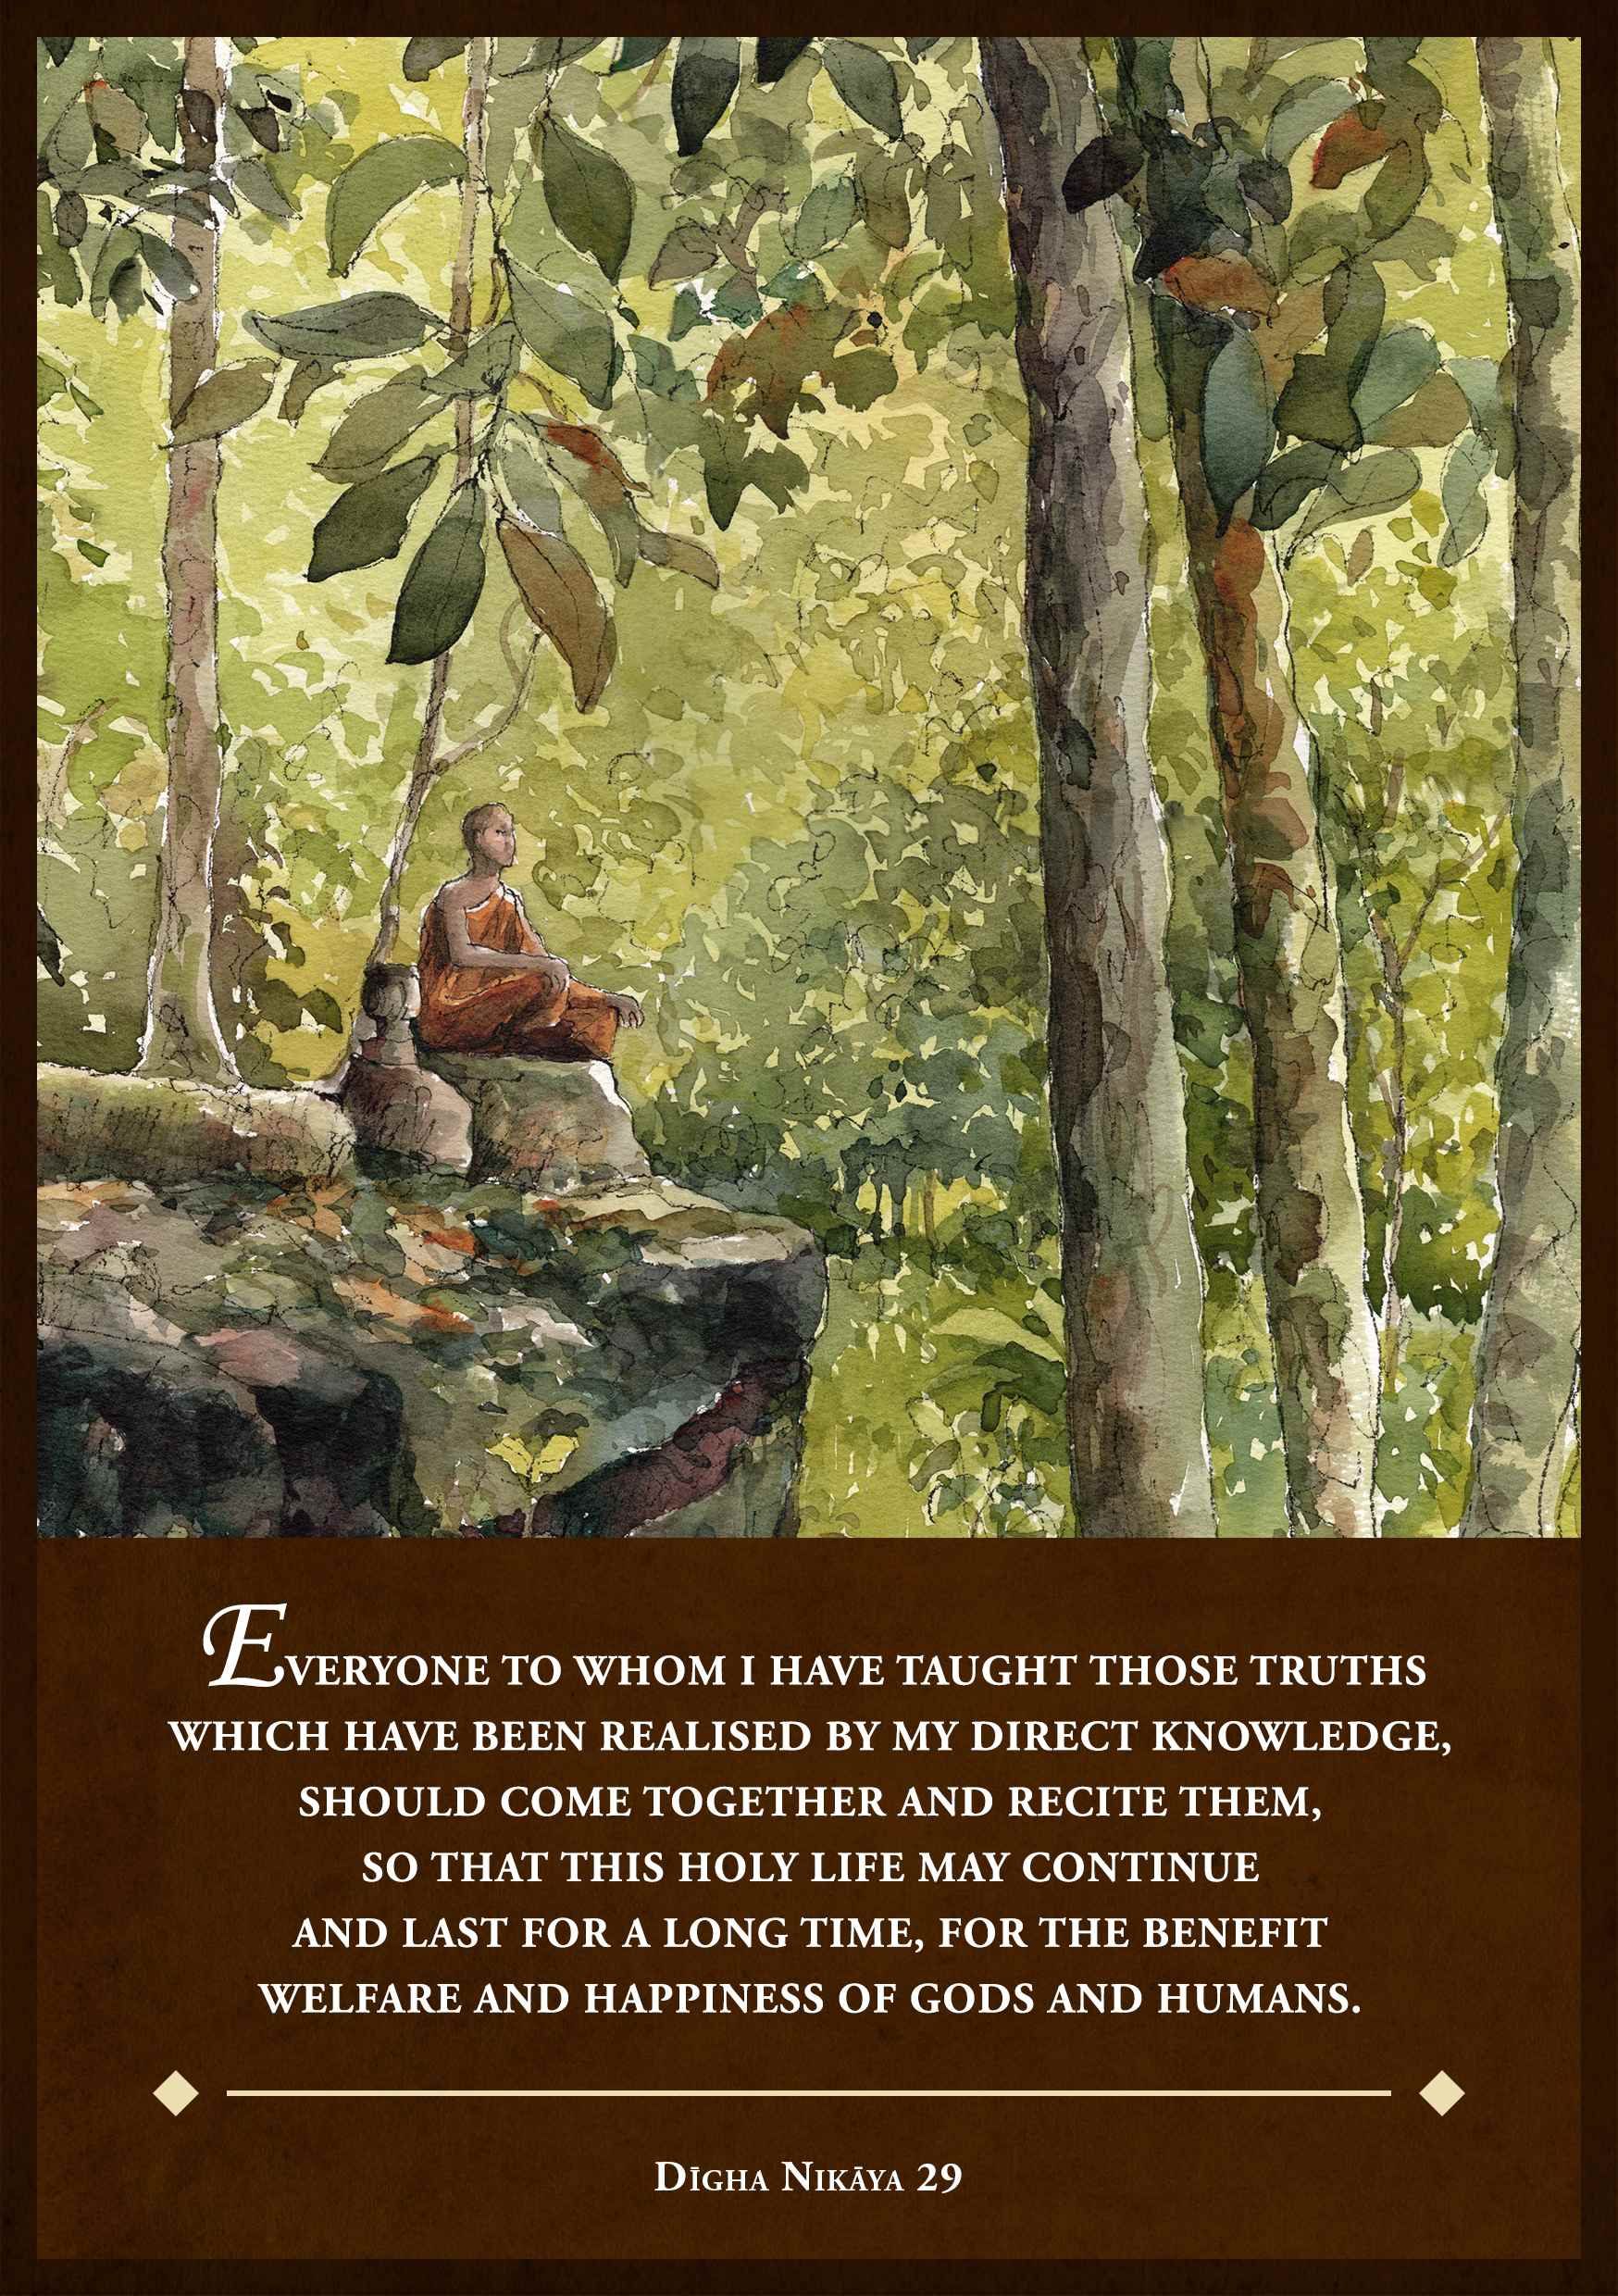
\includegraphics[height=\paperheight]{./back-cover-compressed.jpg}}
\fi

\end{document}
